\documentclass[a4paper,fleqn,usenatbib]{mnras}
\usepackage[T1]{fontenc}
\usepackage{ae,aecompl}


\usepackage{graphicx}	% Including figure files
\usepackage{amsmath}	% Advanced maths commands
\usepackage{amssymb}	% Extra maths symbols
\usepackage{subfig}
\usepackage{array}


\usepackage{multirow}
\usepackage{multicol}
\usepackage{blindtext}
\newcolumntype{?}{!{\vrule width 1pt}}
\newcommand{\Msun}{\,{\rm Mpc}$_{\odot}$\,}
\newcommand{\Mpch}{\,{\rm Mpc}\,\ifmmode h^{-1}\else $h^{-1}$\fi}
\newcommand{\kpch}{\,{\rm kpc}\,\ifmmode h^{-1}\else $h^{-1}$\fi}
\newcommand{\kpc}{\,{\rm kpc}\,}


\newenvironment{Table}
   {\par\bigskip\noindent\minipage{\columnwidth}\centering}
   {\endminipage\par\bigskip}

\title[The shape of dark matter haloes in the Auriga simulations]
{Dark matter halo shape in the Auriga simulations: radial
  dependence, time evolution and correlation with baryon disk
  properties}
\author[Jesus Prada,  Jaime E. Forero-Romero, Volker Springel ]{
Jesus Prada,$^{1}$\thanks{E-mail: jd.prada1760@uniandes.edu.co}
Jaime E. Forero-Romero,$^{1}$
Volker Springel$^{2}$
\\
% List of institutions
$^{1}$Departamento de F\'sica, Universidad de los Andes, Cra. 1 No.
18A-10, Edificio Ip, Bogot\'a, Colombia.\\
$^{2}$Heidelberg Institute for Theoretical Studies,
Schloss-Wolfsbrunnenweg 35, D-69118 Heidelberg, Germany.\\
}

% These dates will be filled out by the publisher
\date{Accepted XXX. Received YYY; in original form ZZZ}

% Enter the current year, for the copyright statements etc.
\pubyear{2018}

% Don't change these lines
\begin{document}
\label{firstpage}
\pagerange{\pageref{firstpage}--\pageref{lastpage}}
\maketitle

% Abstract of the paper
\begin{abstract}
We present shape measurements of dark matter halos in a suit
of 30 cosmological simulations from the Auriga project.
For all measurements we compare the results in full
magnetohydrodynamics against dark matter only physics.
We find a strong influence of baryons in making dark matter halos rounder at all
radii compared to its dark matter only counterparts.
This change in triaxility its more pronounced towards the inner
regions of the halo.
At distances close to the disk rounder dark matter distributions
correlate with massive stellar disks and low gas density.
The dark matter shape shows a strong alignment with the
stellar disk shape as a function of radius, the stronger aligmnet is
found at $~50$kpc, this alignment weakens at smaller and larger radii. 
In dark matter only simulations the time evolution of the shape
measured at the virial radius correlates with the radial shape
evolution at present day.  
However, this correlation is lost once the baryonic effects are
included. 
We conclude that in our simulation suite that baryonic physics
produces rounder halos with a strong correlation between its inner
shape and the stellar and gaseous properties of the disk.
\end{abstract}

% Select between one and six entries from the list of approved keywords.
% Don't make up new ones.
\begin{keywords}
galaxies: evolution --- galaxies: formation --- galaxies: haloes ---
dark matter
\end{keywords}

%%%%%%%%%%%%%%%%%%%%%%%%%%%%%%%%%%%%%%%%%%%%%%%%%%

%%%%%%%%%%%%%%%%% BODY OF PAPER %%%%%%%%%%%%%%%%%%

\section{Introduction}


A robust prediction of the Cold Dark Matter (CDM) paradigm is that DM
halos are ellipsoidal and can be characterized by the principal axes
$a>b>c$.
This ellipsoidal shape is mostly due to the anisotropical and
clumpy accretion of matter influenced by environmental structures.
Numerical studies how that the shape has a strong mass dependence
\citep{Allgood_et_al._2006}, halos are also rounder at the outerskirts
than at the inner part. 
Shape also evolves with cosmic time, halos get
rounder as they evolve.  

There is however a high degree of uncertainty on what is the degree of
uncertainty on the degree of ellipticity of the Milky Way DM halo.
This problem has been addressed both by observations and simulations.
The difficulty in making an observational measurement lies in the
indirect nature of the effect; i.e. the ellipticity can only be
constrained by its effects on quantities such as stellar radial
velocities.
In simulations the uncertainty on predicting the MW DM ellipticity is 
driven by the different physical effects that should be modeled and
its different possible numerical implementations.


Observationally some studies prefer oblate (i.e. a=b>c) configurations at small
distances around $\leq 20$ kpc
\citep[see][]{Law_and_Majewski_2010,Bovy_et_el._2016,Loebman_et_al._2012,Olling_and_Merrifield_2000,Banerjee_and_Chanda_2011} 
and more triaxial and prolate configurations on the outter distances
$\geq 20$ kpc 
\citep[see][]{Vera-Ciro_and_Helmi_2013,Law_and_Majewski_2009,Deg_and_Widrow_2013,Banerjee_and_Chanda_2011}.
However, some  studies are inclined towards prolate configurations even at the inner
parts of the halo \citep[see][]{Bowden_et_al._2016}, and
although it previously seemed that a triaxial DM halo on the
outerskirts would be necessary to fully explain the characterization
of the Sagittarius stream \citep{Law_and_Majewski_2009}, recent studies
questioned this claim by reporting inconsistencies with narrow stellar
streams \citet{Pearson_et_al._2015} or finding that
the relaxation of other constraints may make this claim unnecessary
\citet{Ibata_et_al._2013}. 

In simulations there is strong evidence claiming that the presence of
baryons produces axisymmetrical halos.  
For instance, some studies have shown that the DM halo shape must be
axisymmetrical to ensure the stability of a hydrodynamical disk
embeded in a static DM halo. 
Other have studied this rounding effect by simulating the disk as rigid
potential inside an N-body triaxial DM
halo \cite{Debattista_et_al._2008,Debattista_et_al._2013,Kazantzidis_et_al._2010}
finding that the halo responds to the disk by becoming less triaxial. 

The caveat of the studies mentioned above is that they do not
follow baryons in the whole cosmological context. 
Other studies overcome this limitation by using resimulations 
\citep{Abadi_et_al._2010,Bryan_et_al._2013} finding that the
feeback related to star formation in the disk drives the strenght of
the round effect. 
Recently \cite{2018arXiv180907255C} made a study in a cosmological
simulation to compare the effect of including baryons. They do find,
on average, rounder halo shapes once hydrodynamic effects are
included, but it is uncertain the strenght of this statistical effect
on galaxies similar to the MW.


All these difficulties (enough numerical resolution, explicit
cosmological context, appropriate feedback physics to produce
realistic MW disks) have limited the studies that want to study the
rounding effect of baryons in MW-like galaxies.
In this work we overcome all these limitations by analyzing the
results of state-of-the-art hydrodynamical simulations of isolated
halos that resemble the Milky Way.
We also perform a convergence study with simulation performed at
different resolution levels and explicitly compare the role of DM only
vs. DM+hydro on the MW DM halo shape.


\section{Numerical Simulations}


The Auriga project offers cosmological zoom in simulations of MW-sized 
dark matter halos in a $\Lambda$CDM cosmology. 
This simulations come in two versions: dark matter only and
baryonic physics including magetohydrodynamics (MHD).
A detailed description of the simulations and their
disk properties can be founc in \citep{auriga}, here we summarize its
main features.

The objects in those simulations were selected from a set of 30
isolated halos in the Evolution and Assembly of GaLaxies and their
Environments (EAGLE)  project \citep{Eagle}.   
These halos were randomly selected from a sample of the most isolated
halos at $z=0$ whose virial mass $M_{200}$ was between $10^{12}M_\odot$ and
$2\times 10^{12}M_\odot$. 
The cosmological parameters in these simulatins correspond to
$\Omega_m=0.307$, $\Omega_b=0.048$, $\Omega_\Lambda=0.693$ and a
dimensionless Hubble parameter $h=0.6777$ [CITATION PLANCK 2014]


The selected halos were re-simulated at higher resultion by applying a
zoom-in technique with varying physical realism using the moving-mesh AREPO code
that includes gravity, ideal magnetohydrodynamics (MHD), 
phenomenological descriptions for star formation, chemical enrichment
from supernovae and its stellar feedback.  The simulation also follows
the formation and evolution of black holes together with the Active
Galactic Nuclei feedback \citep{arepo} [CITATIONPAKMORE].  


The 30 zoom-in halos have a dark matter particle mass of $\sim 3\times
10^5$\Msun while the barynic mass resolution is $\sim 5\times 10^4$\Msun.
The softening lenght for gravitational force computation for stellar
particles and high-resolution dark matter particles 
is fixed to be 500 $h^{-1}$ pc in comoving coordinates up to $z=1$,
and 396 pc in physical coordinates afterwards.
The gravitational softening lenght for gas cells changes with the mean
cell radius but is limited to be larger than the stellar softening
lenght and 1850 pc physical. 
This setup corresponds to \texttt{Level4} resolution.
From these 30 halos, 6 of them where re-simulated at higher resolution
taking into account a spatial factor of 2 in each spatial dimension,
this is the \texttt{Level3} resolution.  
There are $\sim 4\times 10^6$ dark matter particles within the virial radius
of \texttt{Level4} halos at $z=0$, this number increases to $\sim 3\times 10^7$ in
\texttt{Level3} simulations. 
 
In this work all the results that we report at $z=0$ as a function of radius and
the correlations with disk properties correspond to the 30 halos in
the \texttt{Level4} resolution. 
For the measurement on shape evolution with time we use the 6 halos in
the \texttt{Level3} simulations.
Finally, all  halos described so far have also been simulated at the same
resolutions without MHD using dark matter particles only, we refer to
these halos as the DMO (Dark Matter Only) sample.



\begin{figure*}
  \centering
  \subfloat[DMO simulation. Shape at small radius.]{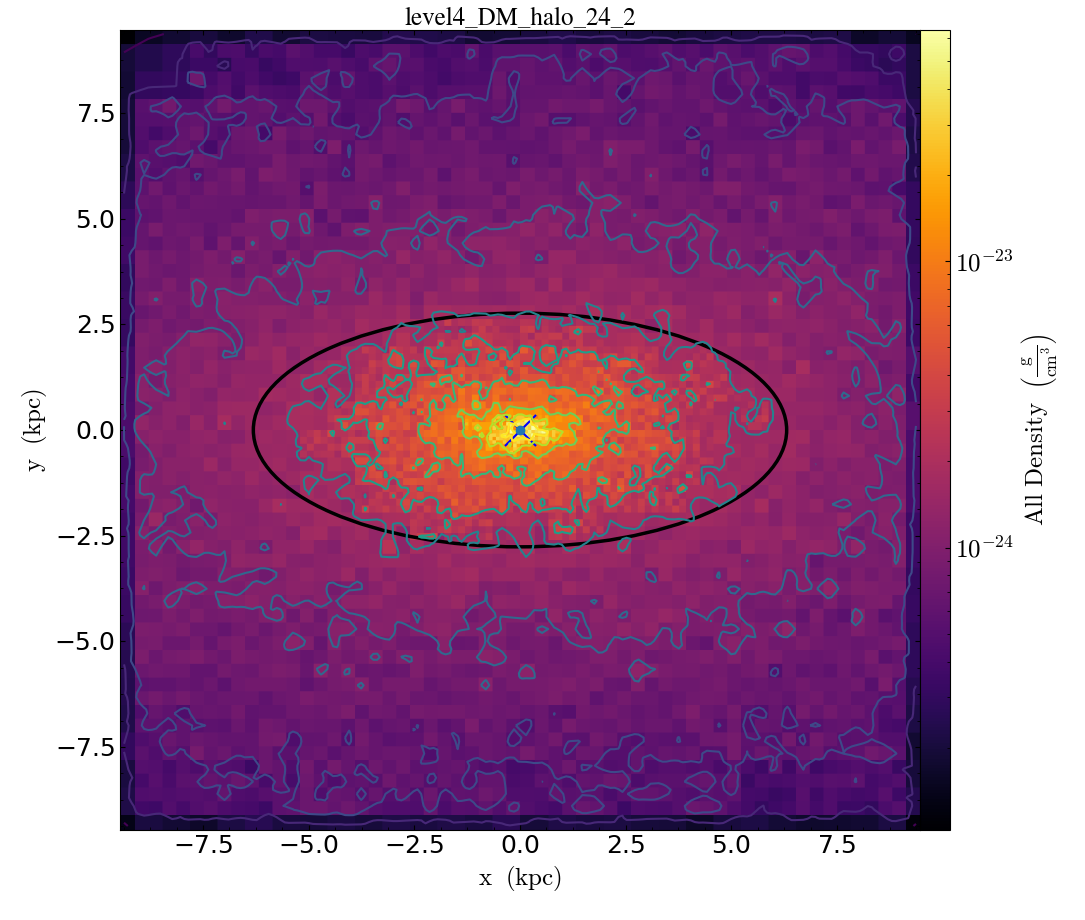
\includegraphics[width=0.5\textwidth]{level4_DM_halo_24_2.png}} 
  \hfill
  \subfloat[DMO simulation. Shape at large radius.]{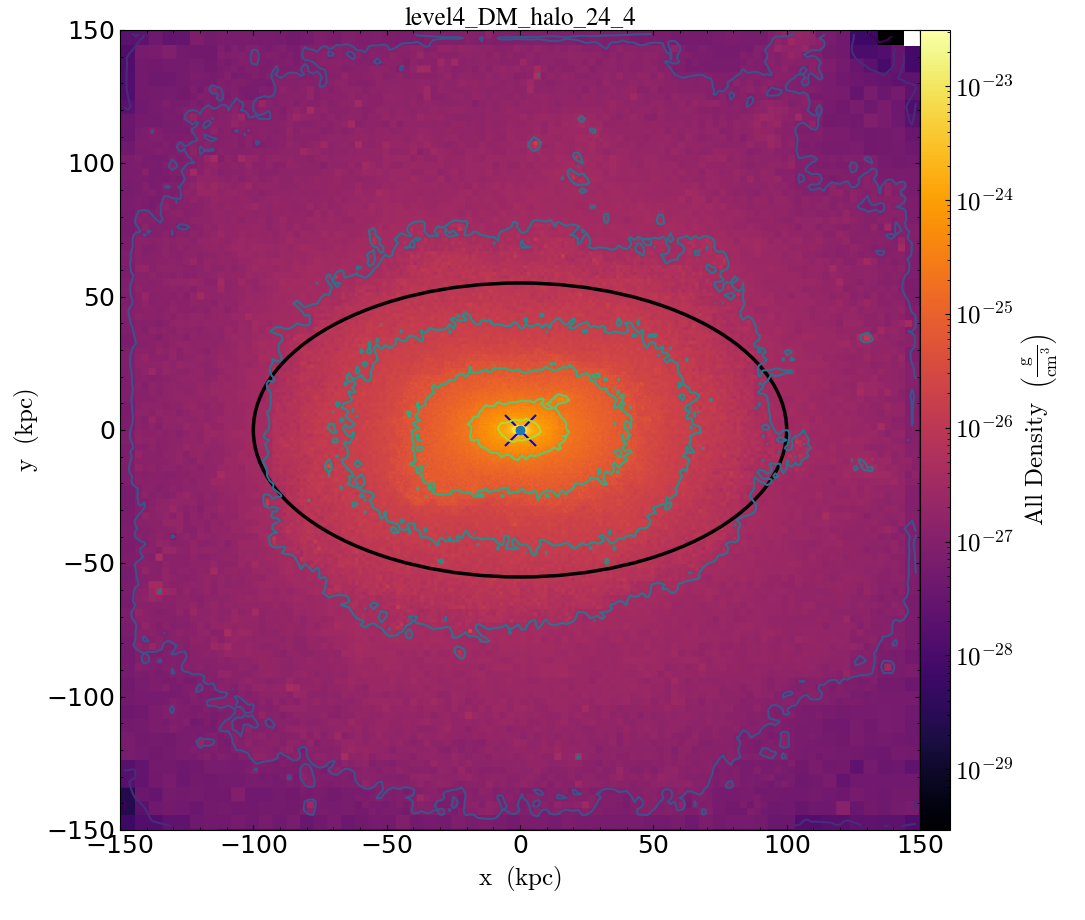
\includegraphics[width=0.5\textwidth]{level4_DM_halo_24_4.png}} 
  \hfill 

  \subfloat[MHD simulation. Shape at small radius.]{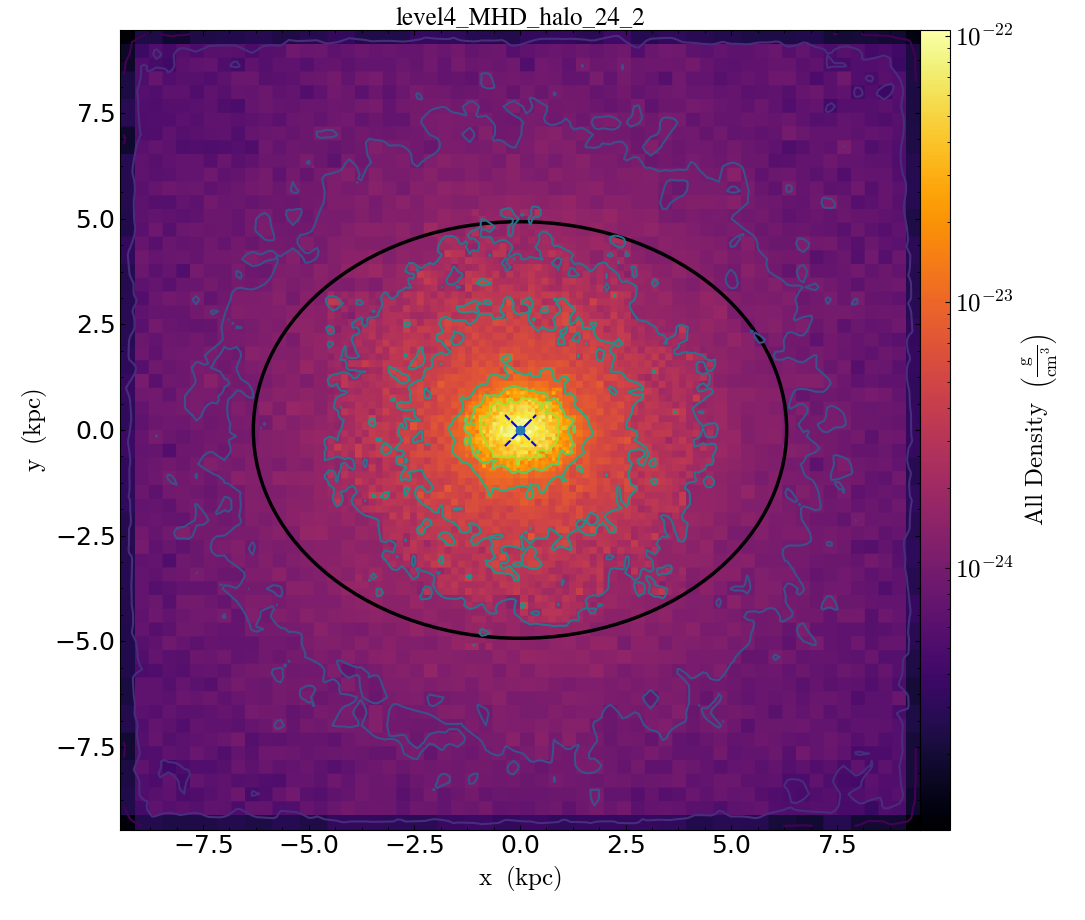
\includegraphics[width=0.5\textwidth]{level4_MHD_halo_24_2.png}} 
  \hfill
  \subfloat[MHD simulation. Shape at large radius.]{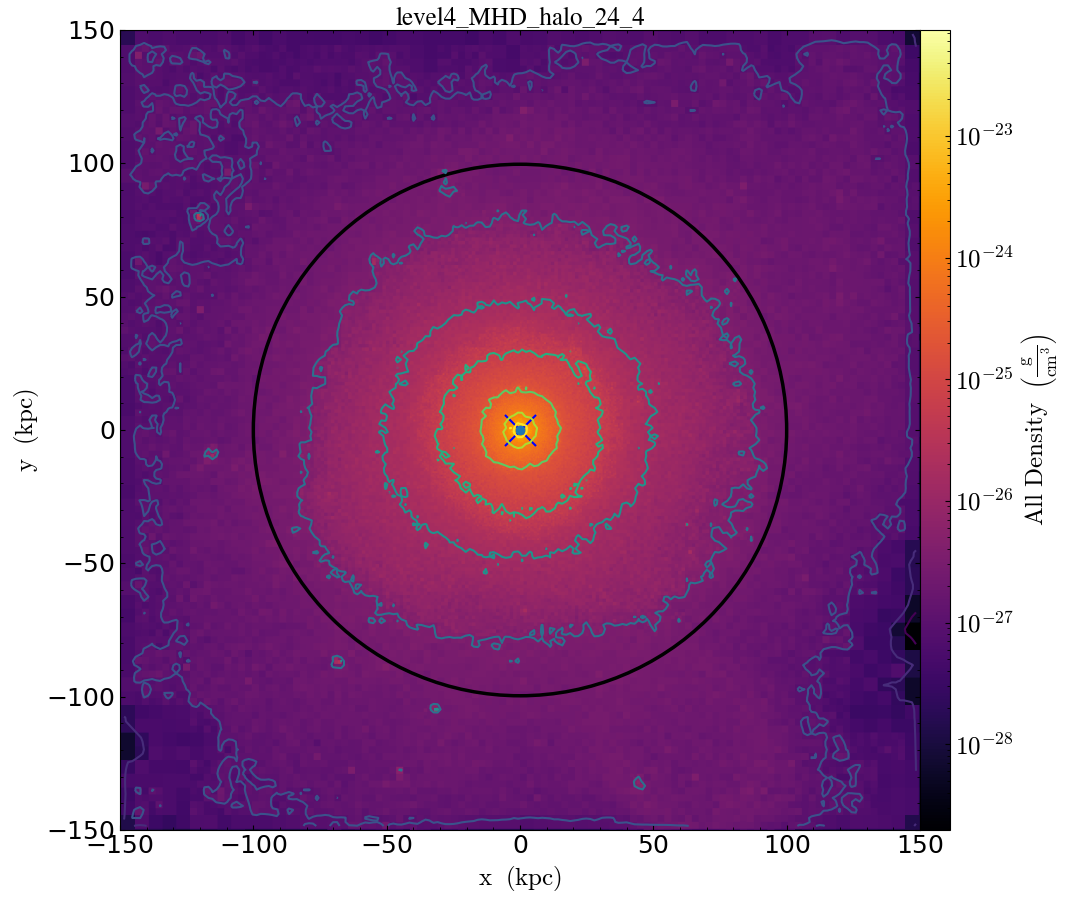
\includegraphics[width=0.5\textwidth]{level4_MHD_halo_24_4.png}} 
  \hfill 
  \caption{DM density in logarithmic scale within a slice of one tenth
    of the virial radius in width. 
    The cut is perpendicular to the short axis of the inertia tensor ellipsoid.
    The black ellipses show the results of the fitting procedure. 
    Upper panels correspond to DMO simulations, lower panels to MHD
    simulations.
    All cases correspond to \texttt{Level4} resolution.
    Left panels show data at small radii, while right panels at large
    radii.    
    This halo showcases the most noticeable effect in all halos
    across the Auriga simulations: DM halos are rounder at all radii
    after baryonic physics is included.}
\label{fig:slices}
\end{figure*}


 
\begin{figure*}
\begin{center}
\subfloat[DMO simulations.]{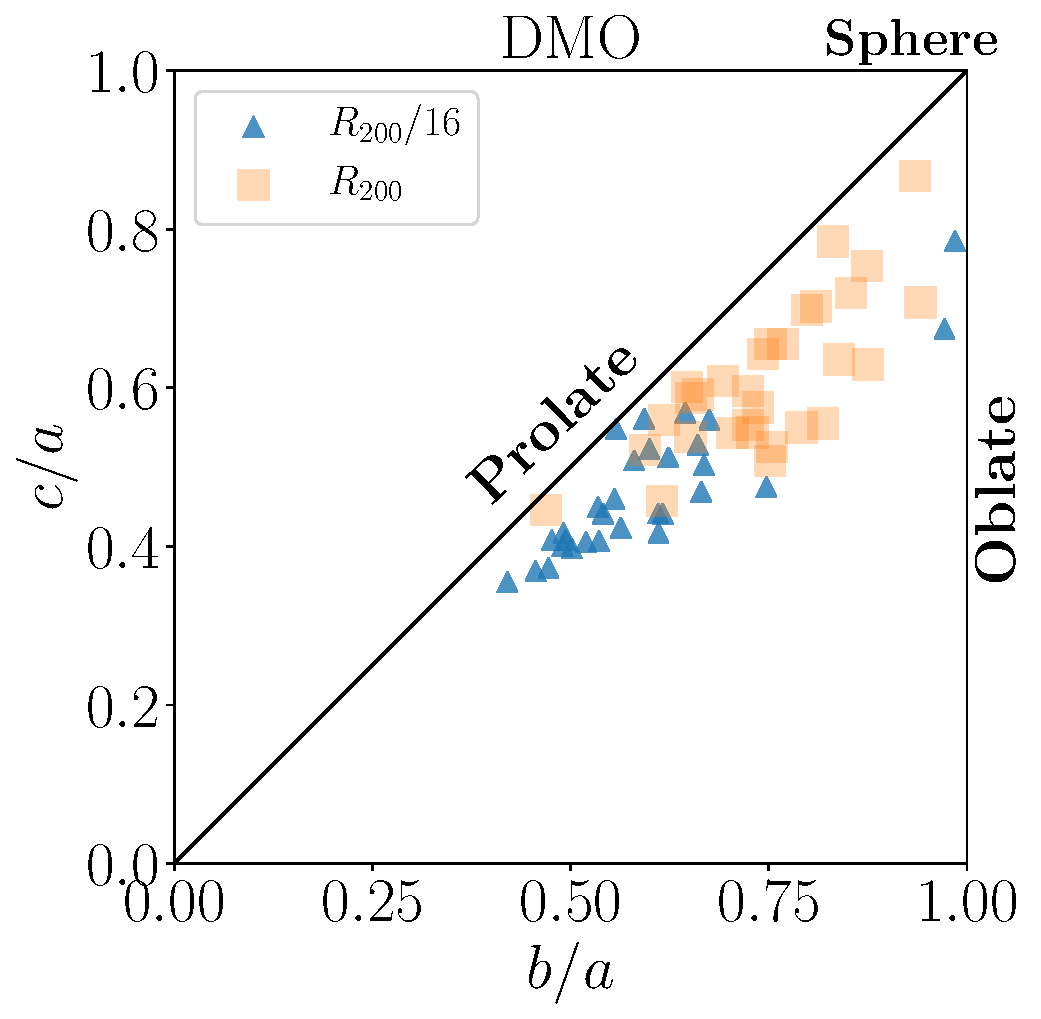
\includegraphics[width=0.9\columnwidth]{Lvl_4_Triax_Plane_DM.pdf}}
\subfloat[MHD simulations.]{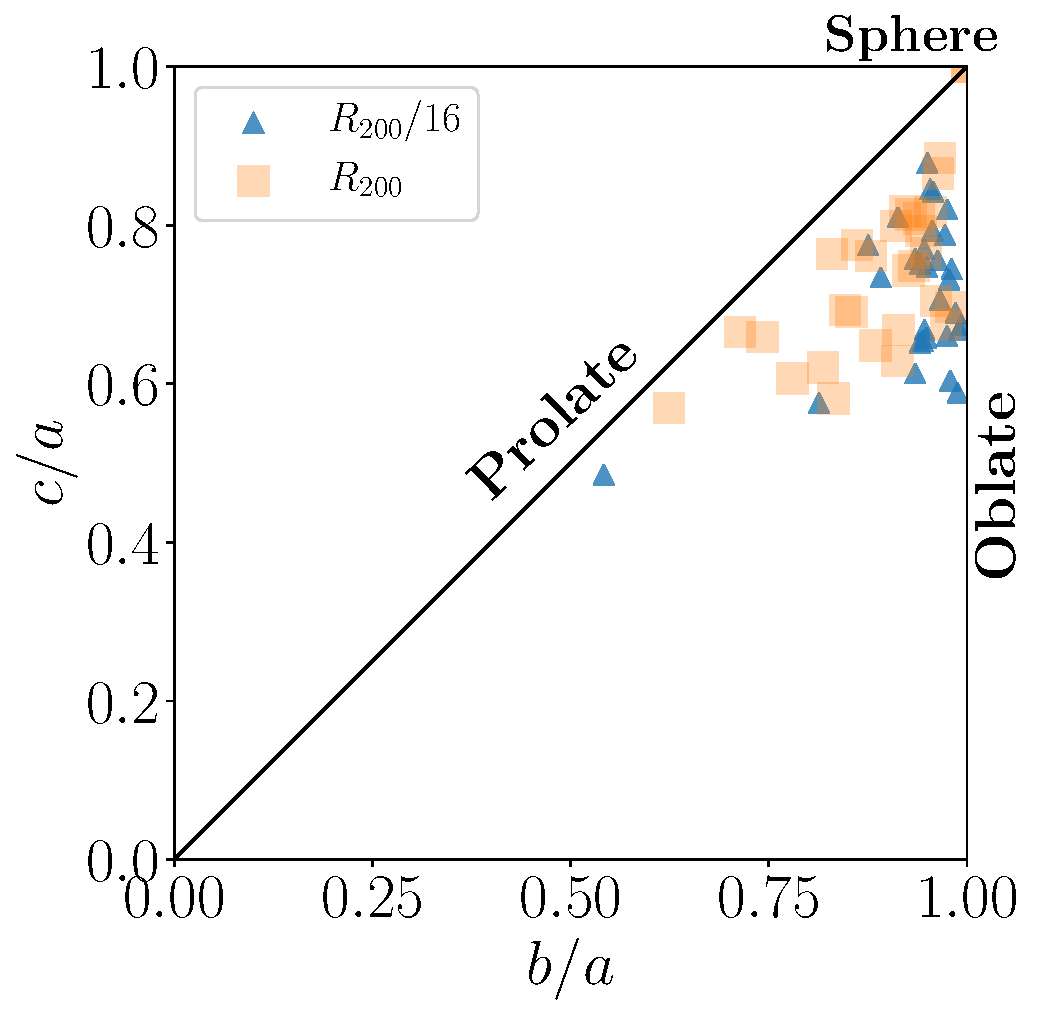
\includegraphics[width=0.9\columnwidth]{Lvl_4_Triax_Plane_MHD.pdf}}
\end{center}
\caption{Axial ratios for all halos in the simulation.
  Left/right panels correspond to DMO/MHD simulations, respectively.
  Triangles (squares) represent the measurements at $R_{200}/16$
  ($R_{200}$) which correspond to physical distances of $14\pm 1$ kpc
  ($230\pm 15$ kpc) respectively.
  Here we can visualize three main trends for the whole halo population.
  First, in DMO simulations halos are rounder in the outskirts
  than in the inner part.
  Second, halos in MHD are rounder than its DMO counterparts.
  Third, halos in MHD are less triaxial in the inner regions than in
  the outskirts.}
  \label{fig:triaxiality_plane}
\end{figure*}


\begin{figure*}
\subfloat[DMO simulations.]{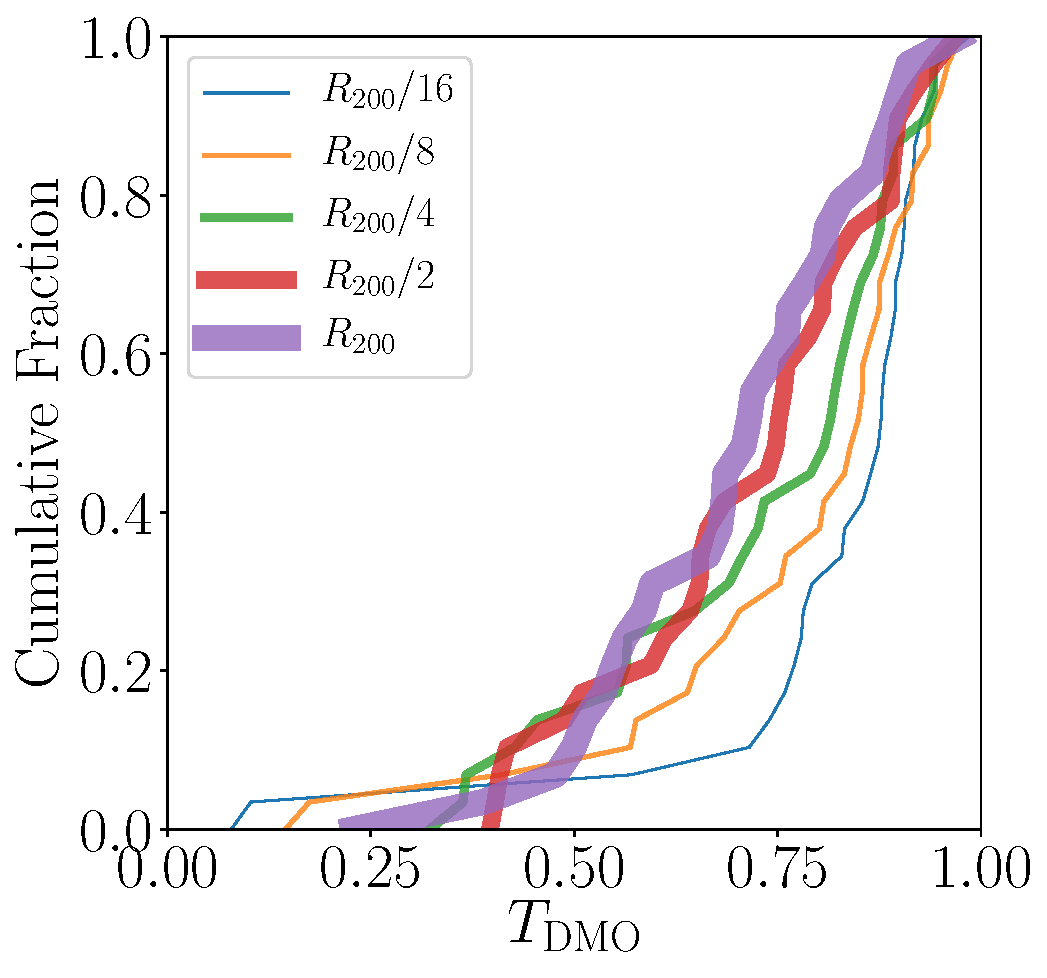
\includegraphics[width=0.9\columnwidth]{triaxialiy_distro_DM.pdf}}
\subfloat[MHD simulations.]{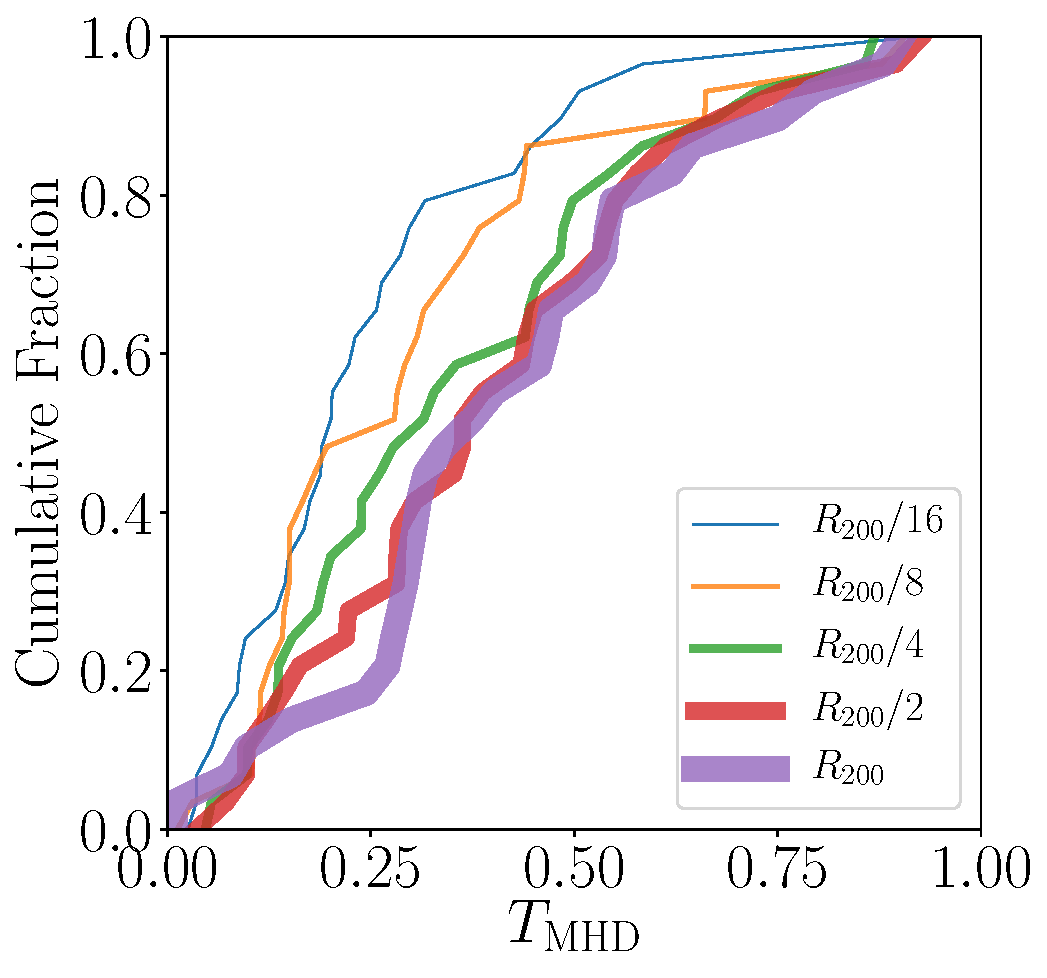
\includegraphics[width=0.9\columnwidth]{triaxialiy_distro_MHD.pdf}}
\caption{Cumulative distribution for the triaxiality at five different radii.
  Right/left panel correspond to DMO/MHD simulations, respectively. 
  In DMO simulations the median triaxiality at all radii is larger
  than $0.5$; only for $20\%$ the triaxility is smaller than $0.5$.
  Furthermore, the triaxility increases as one moves towards the inner
  part of the halo.
  In MHD simulations the situation is reversed.
  The median triaxility at all radii is smaller than $0.5$.
  Moving towards the stellar disk the triaxility decreases towards a median
  value of $T=0.15$.}
\label{fig:triaxial_cumulative}
\end{figure*}


\begin{figure}
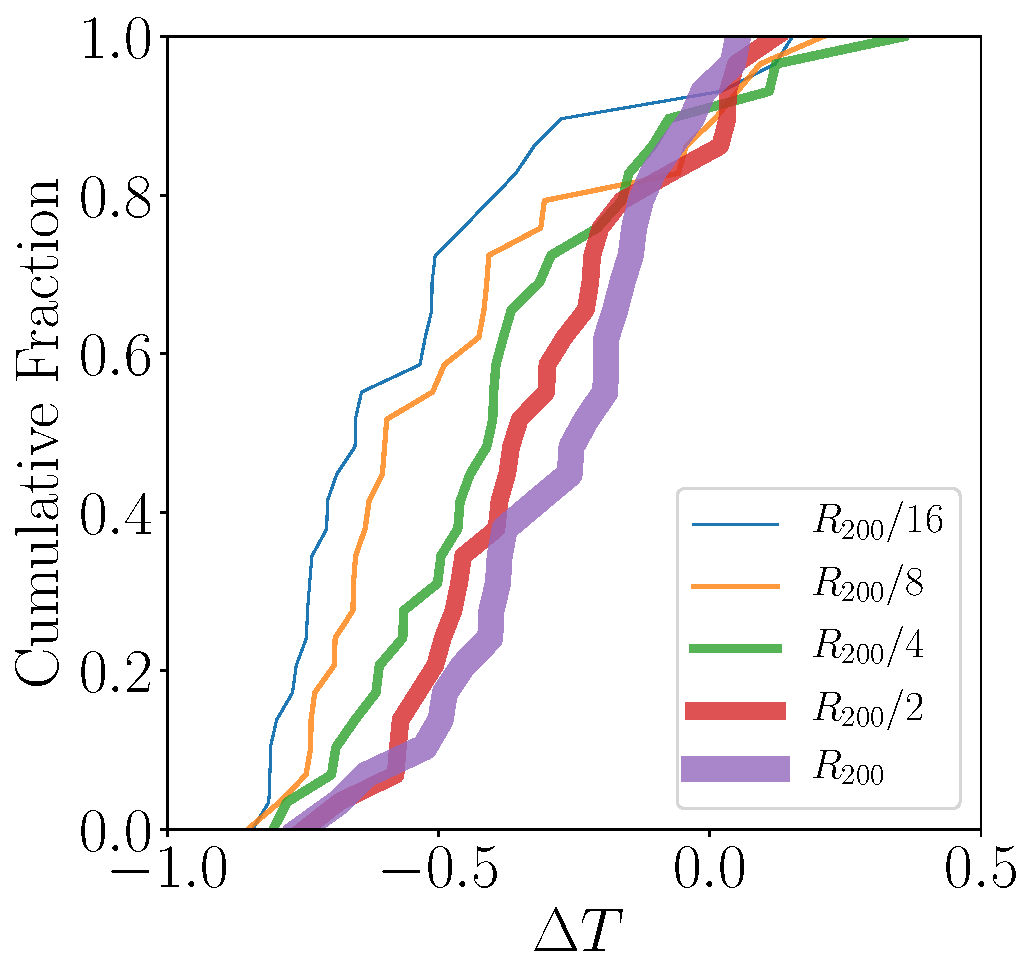
\includegraphics[width=0.9\columnwidth]{delta_triaxiality_distro.pdf}
\caption{
  Cumulative distribution for the change in triaxility $\Delta T=T_{\rm
    MHD}-T_{\rm DMO}$ for the same radii used in Figure
  \ref{fig:triaxial_cumulative}. 
  At the virial radius all the halos become less triaxial in the MHD
  simulations. 
  The change in triaxility becomes stronger in the inner regions of
  the dark matter halo.}
\label{fig:delta_triaxial_cumulative}
\end{figure}


\begin{figure*}
\begin{center}
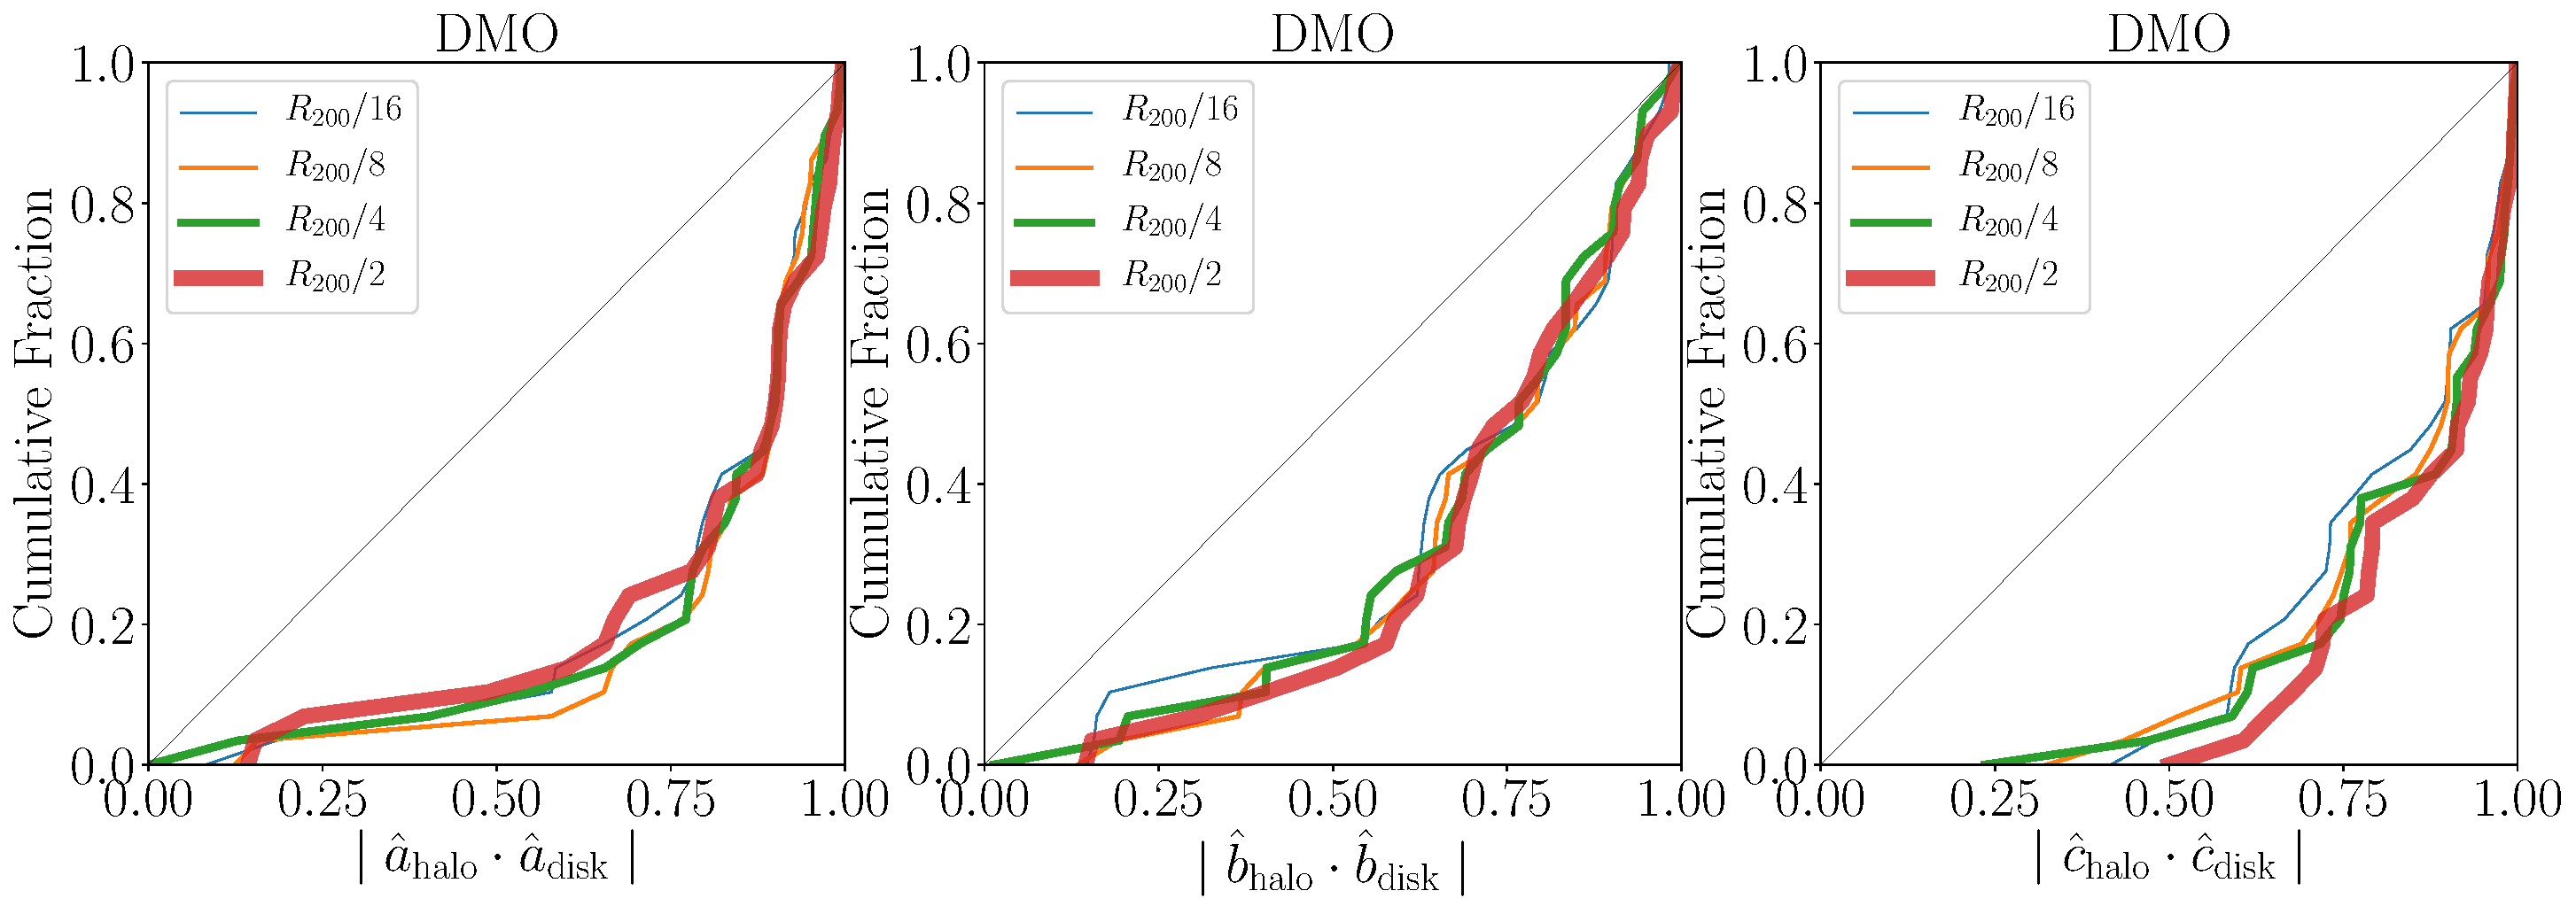
\includegraphics[width=1.0\textwidth]{cumulative_alignment_DM.pdf}
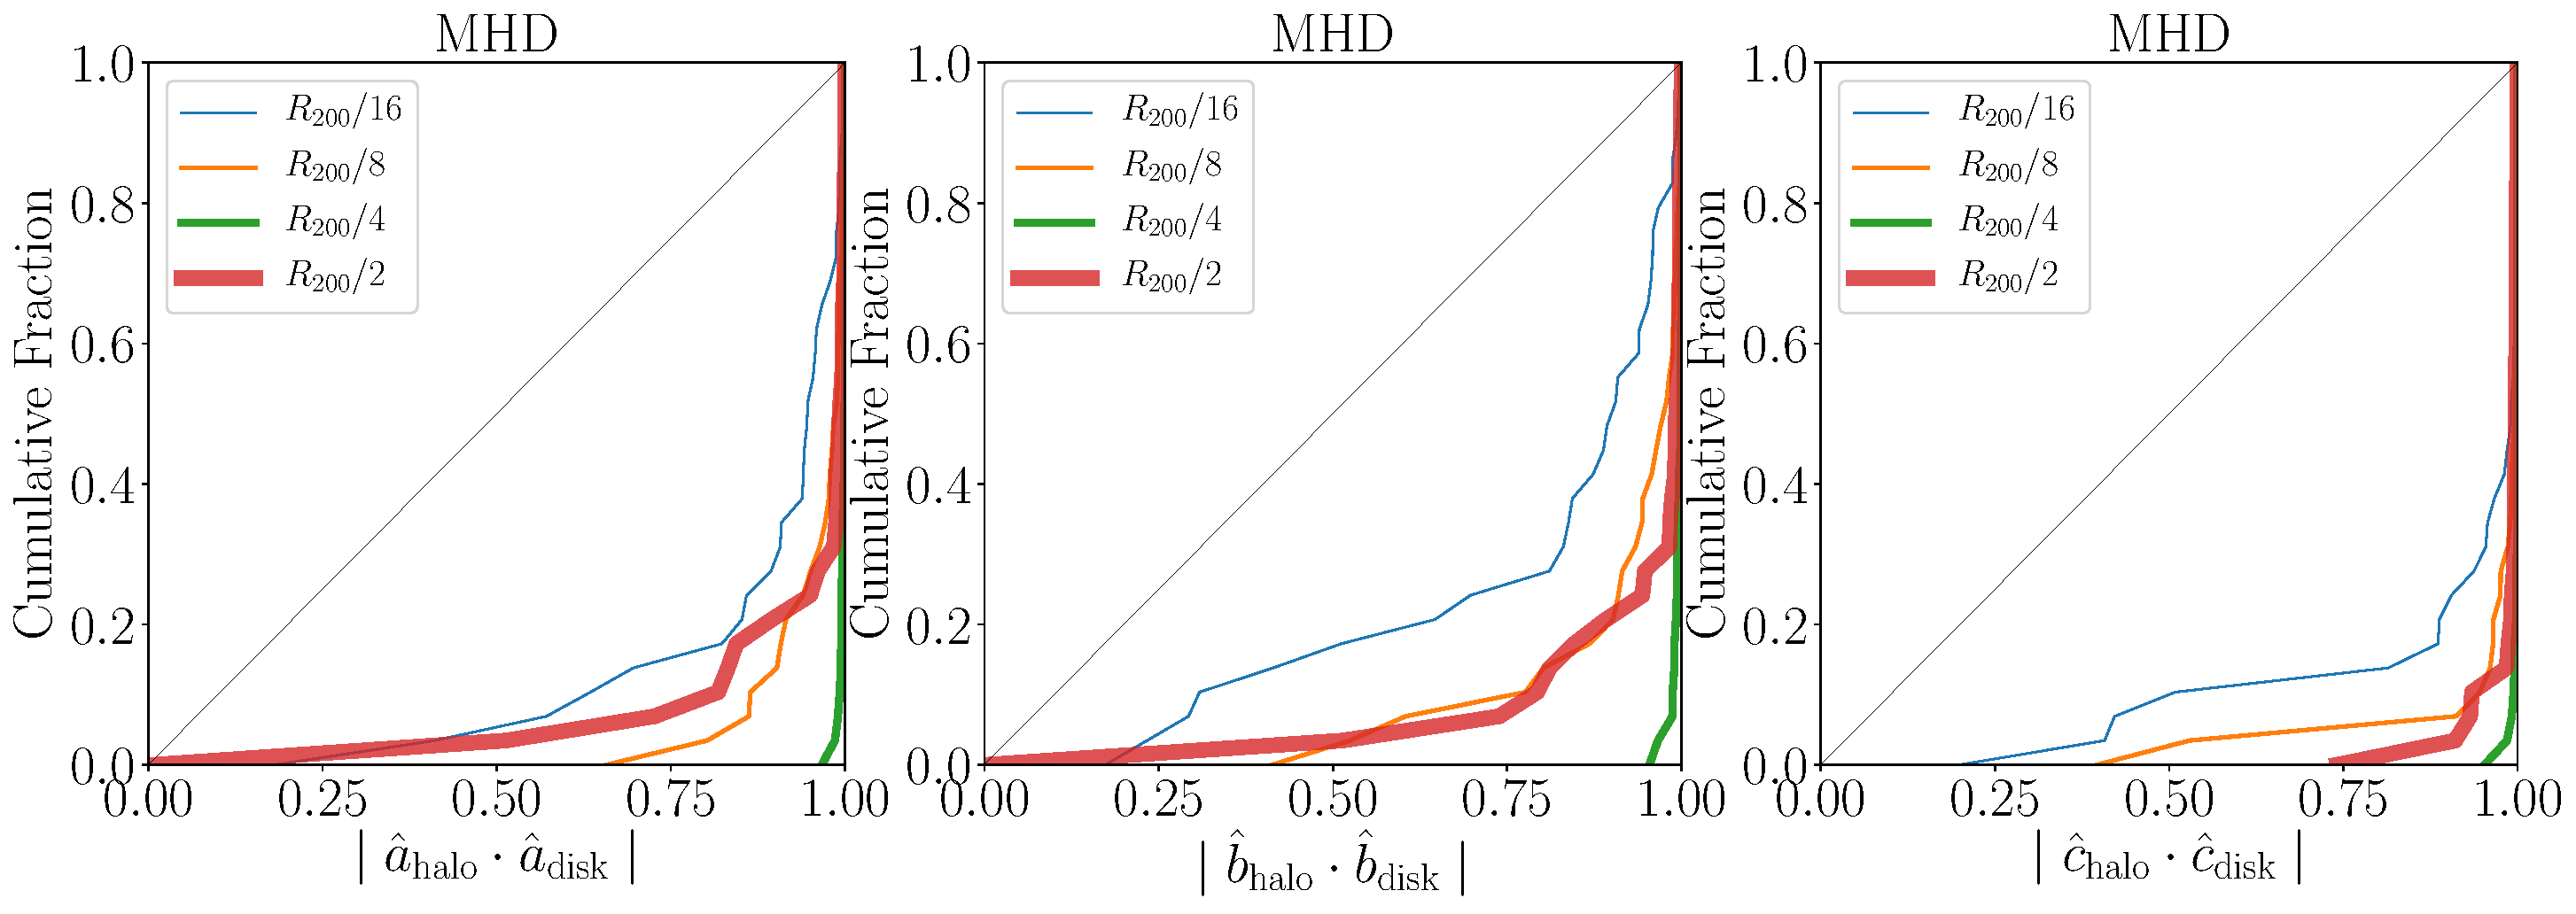
\includegraphics[width=1.0\textwidth]{cumulative_alignment_MHD.pdf}
\end{center}
\caption{Cumulative distribution for the alignments between the
  principal axis of the halo shape and the principal axis of the
  stellar disk in the MHD simulations for radii $\leq 0.5R_{200}$.
  Each panel compares the alingment of the corresponding
  major/middle/minor axis both in the halo and the stellar disk.
  In the upper row the haloes come from the DMO simulation, 
  here the central message is that the shells are aligned to each
  other at every radii.
  In the lower row the haloes come from the MHD simulation and is a
  self-consistent comparison with the disks. 
  In this case the dark matter shells twist and  the degree of the
  halo-disk alignment changes with distance.
  The worst halo-disk alignment happens closer to the disk ($14\pm1$ kpc).
  Interestingly an almost perfect halo-disk alignment happens at an intermediate
  radius of $0.25R_{200}$ ($56\pm 4$kpc); while at a larger
  distance $0.5R_{200}$ the two start to missalign.
}
\label{fig:cumulative_alignment}
\end{figure*}


\begin{figure*}
\begin{center}
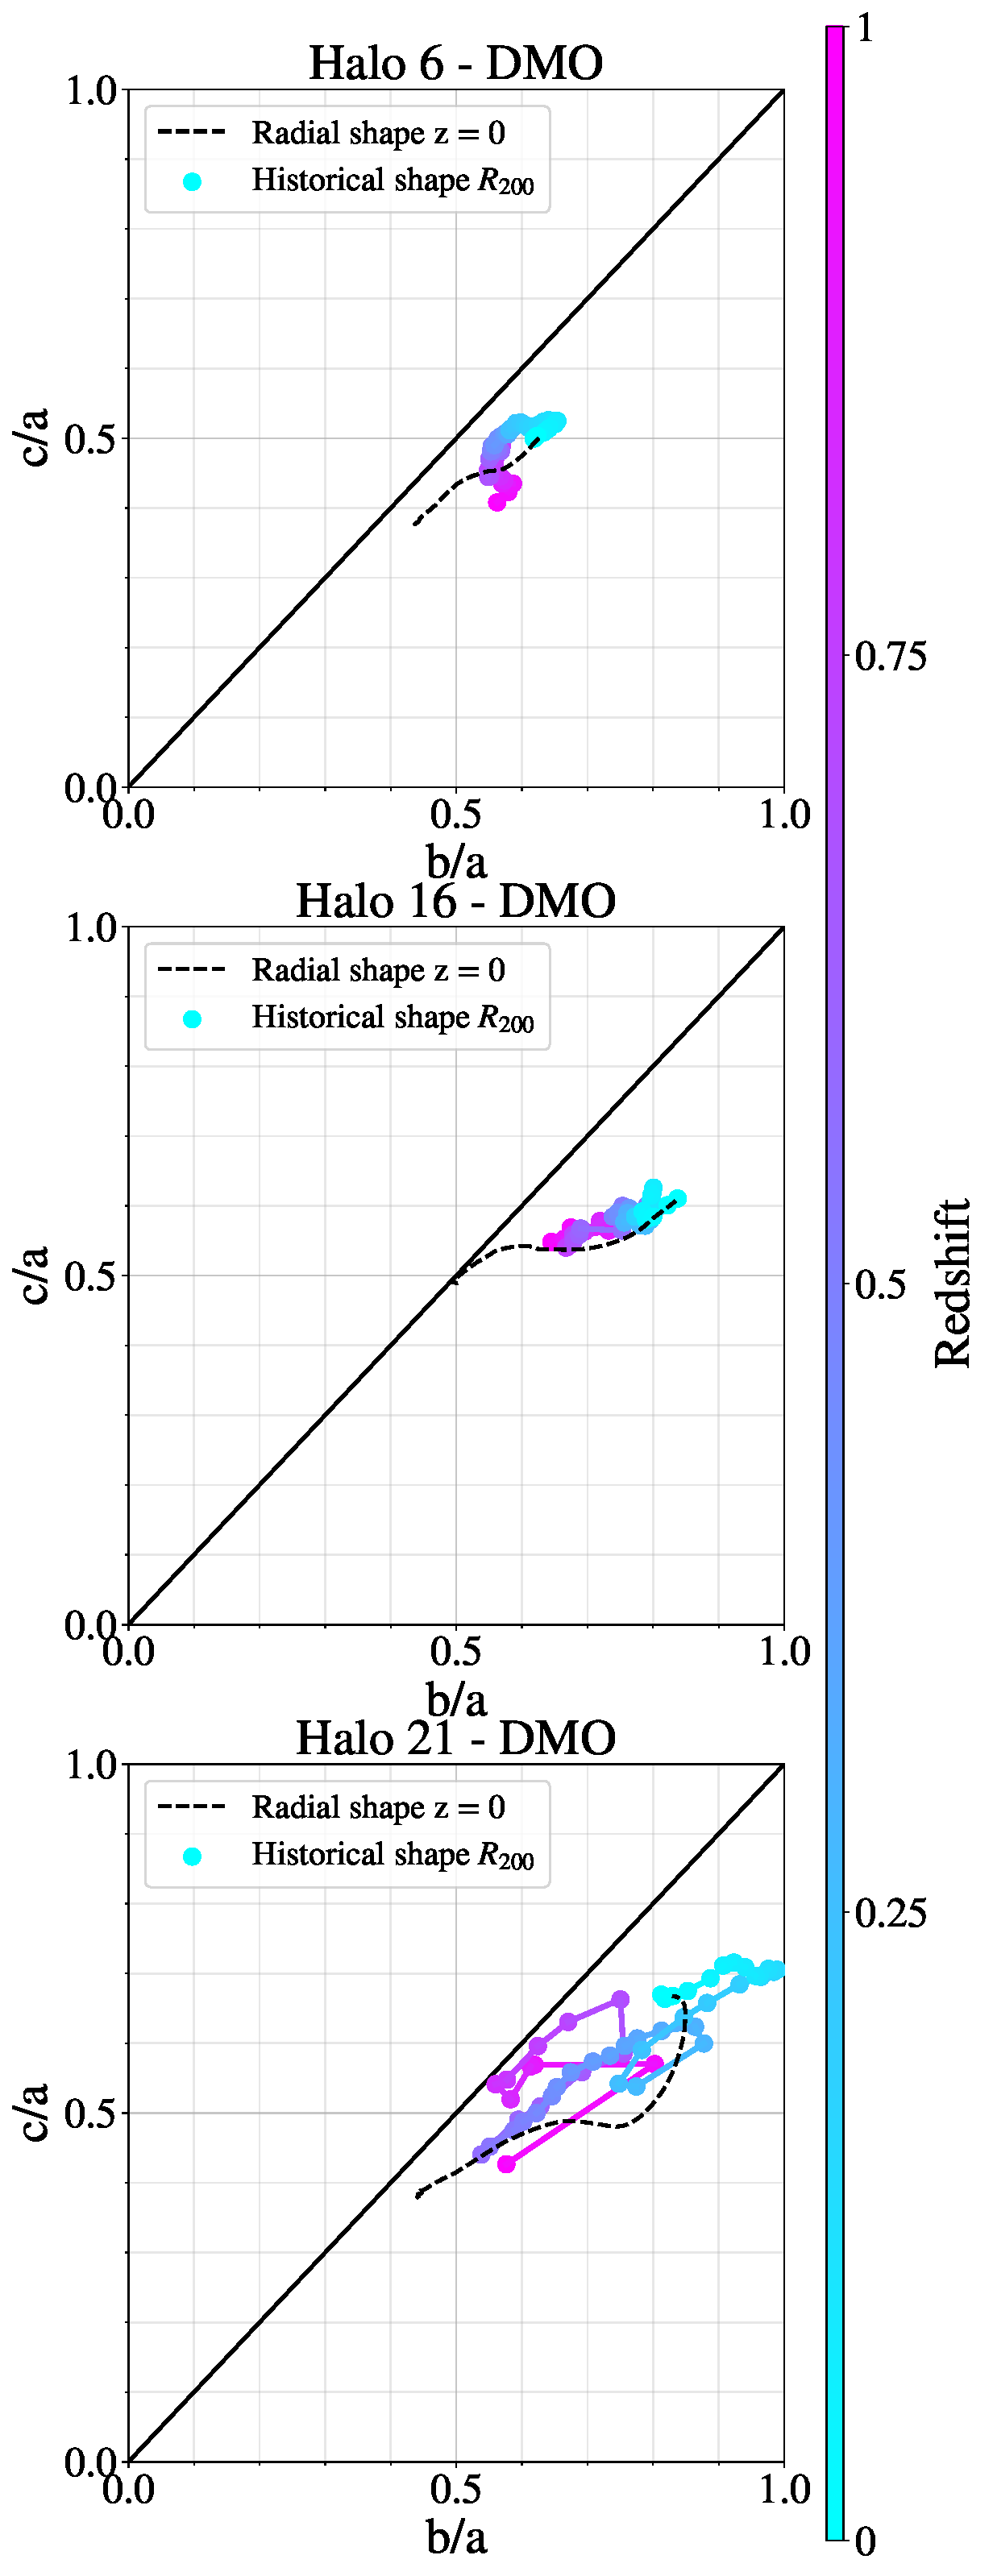
\includegraphics[width=0.35\textwidth]{Z_Triax_level3_set_A_DM.pdf}
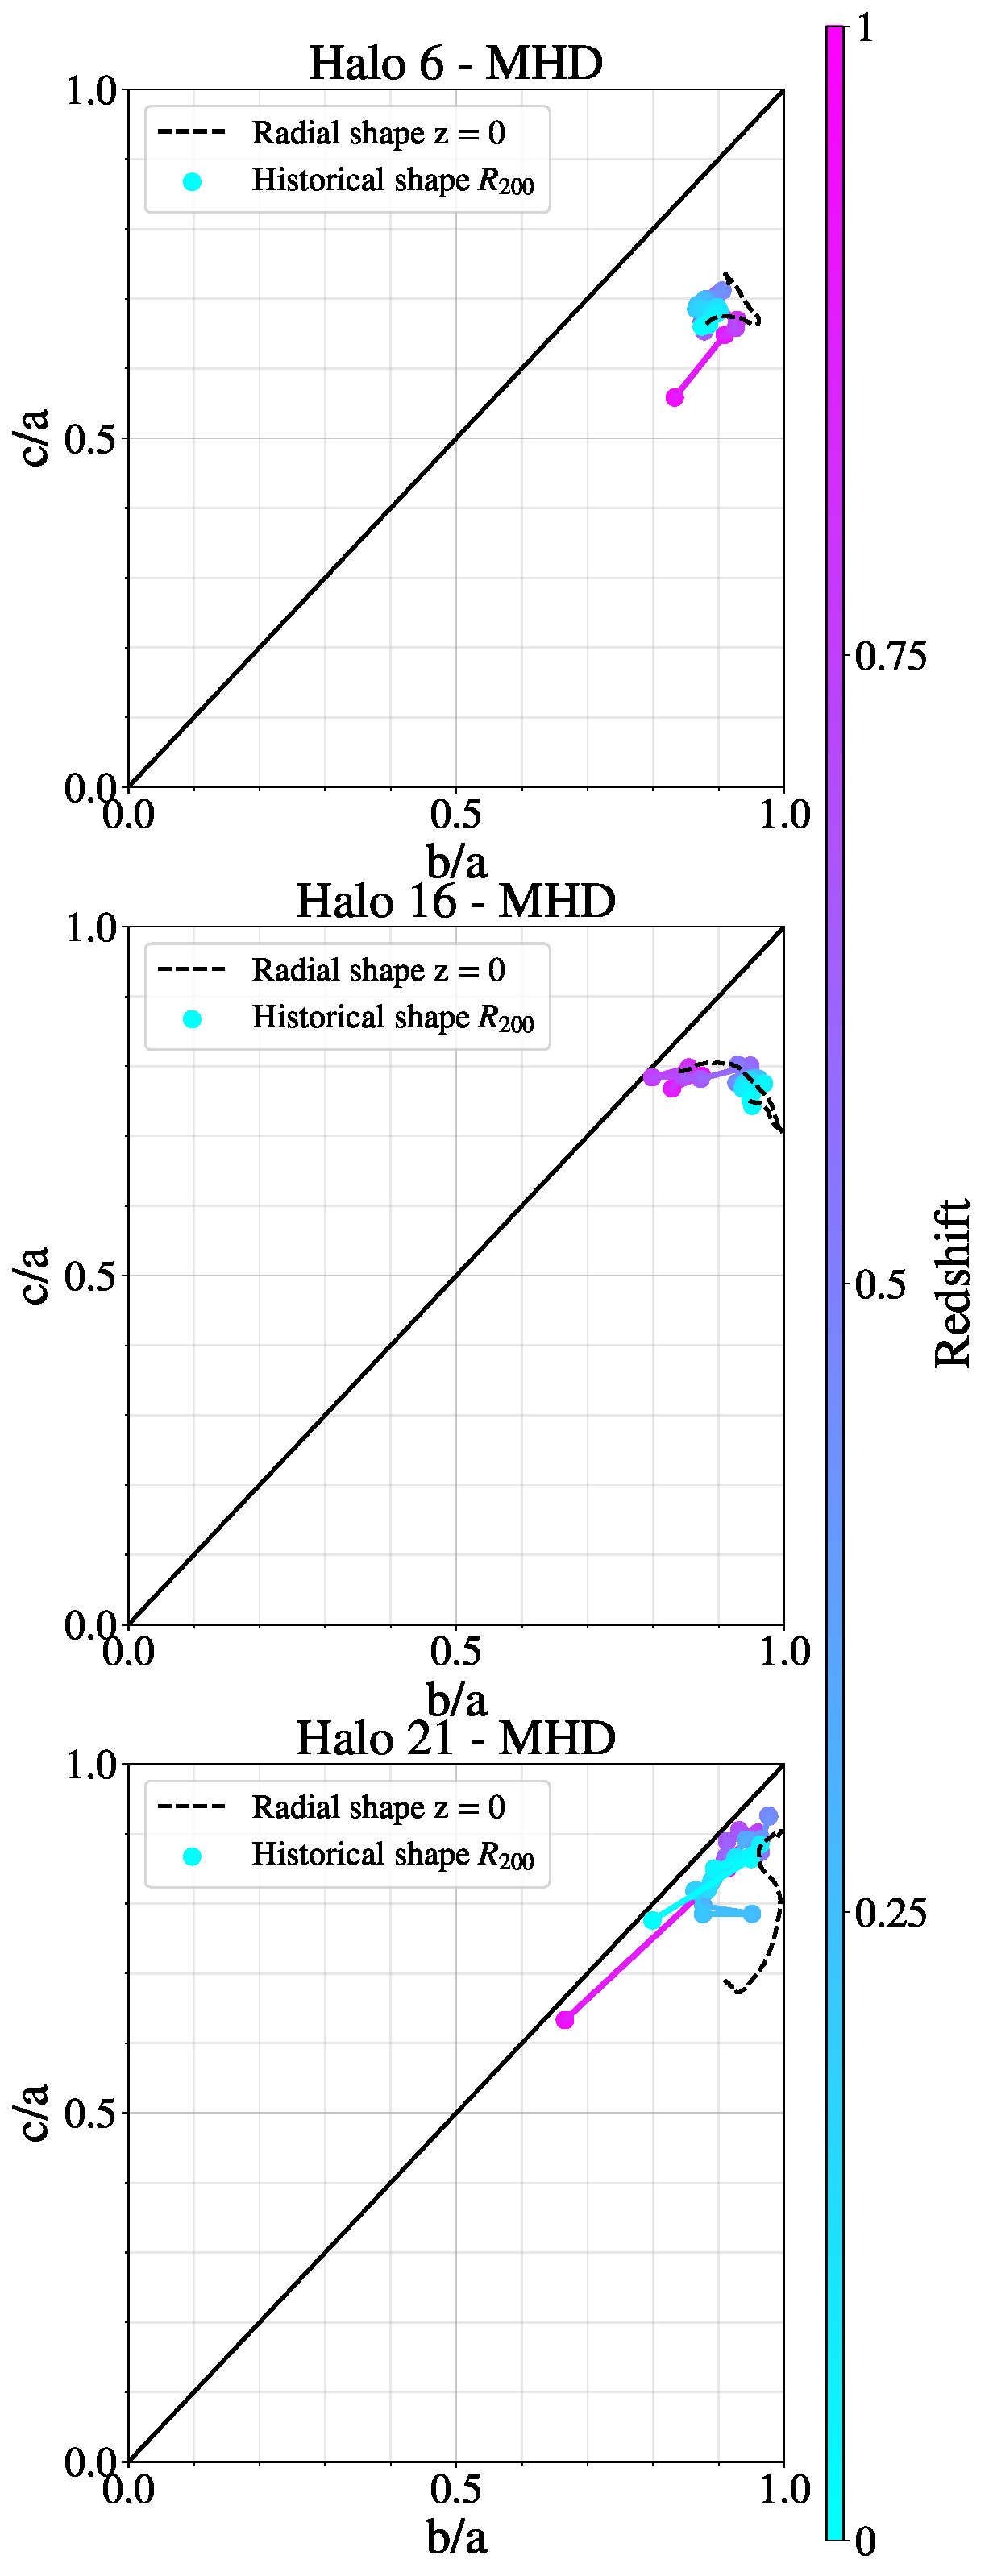
\includegraphics[width=0.35\textwidth]{Z_Triax_level3_set_A_MHD.pdf}
\end{center}
\caption{Axial ratios as a function of time (colour circles) and
  radius (dashed lines). 
  The left/right columns correspond to DMO/MHD simulations, respectively. 
  The colour indicates the redshift at which the shape was measured
  (always at $R_{200}$ at that time.)
  The radial shapes goes from $R_{200}$ down to $\sim 1$ kpc.
  These three halos correspond to a first half the sample for the \texttt{Level3}
  haloes. 
}
\label{fig:triaxial_history_A}
\end{figure*}


\begin{figure*}
\begin{center}
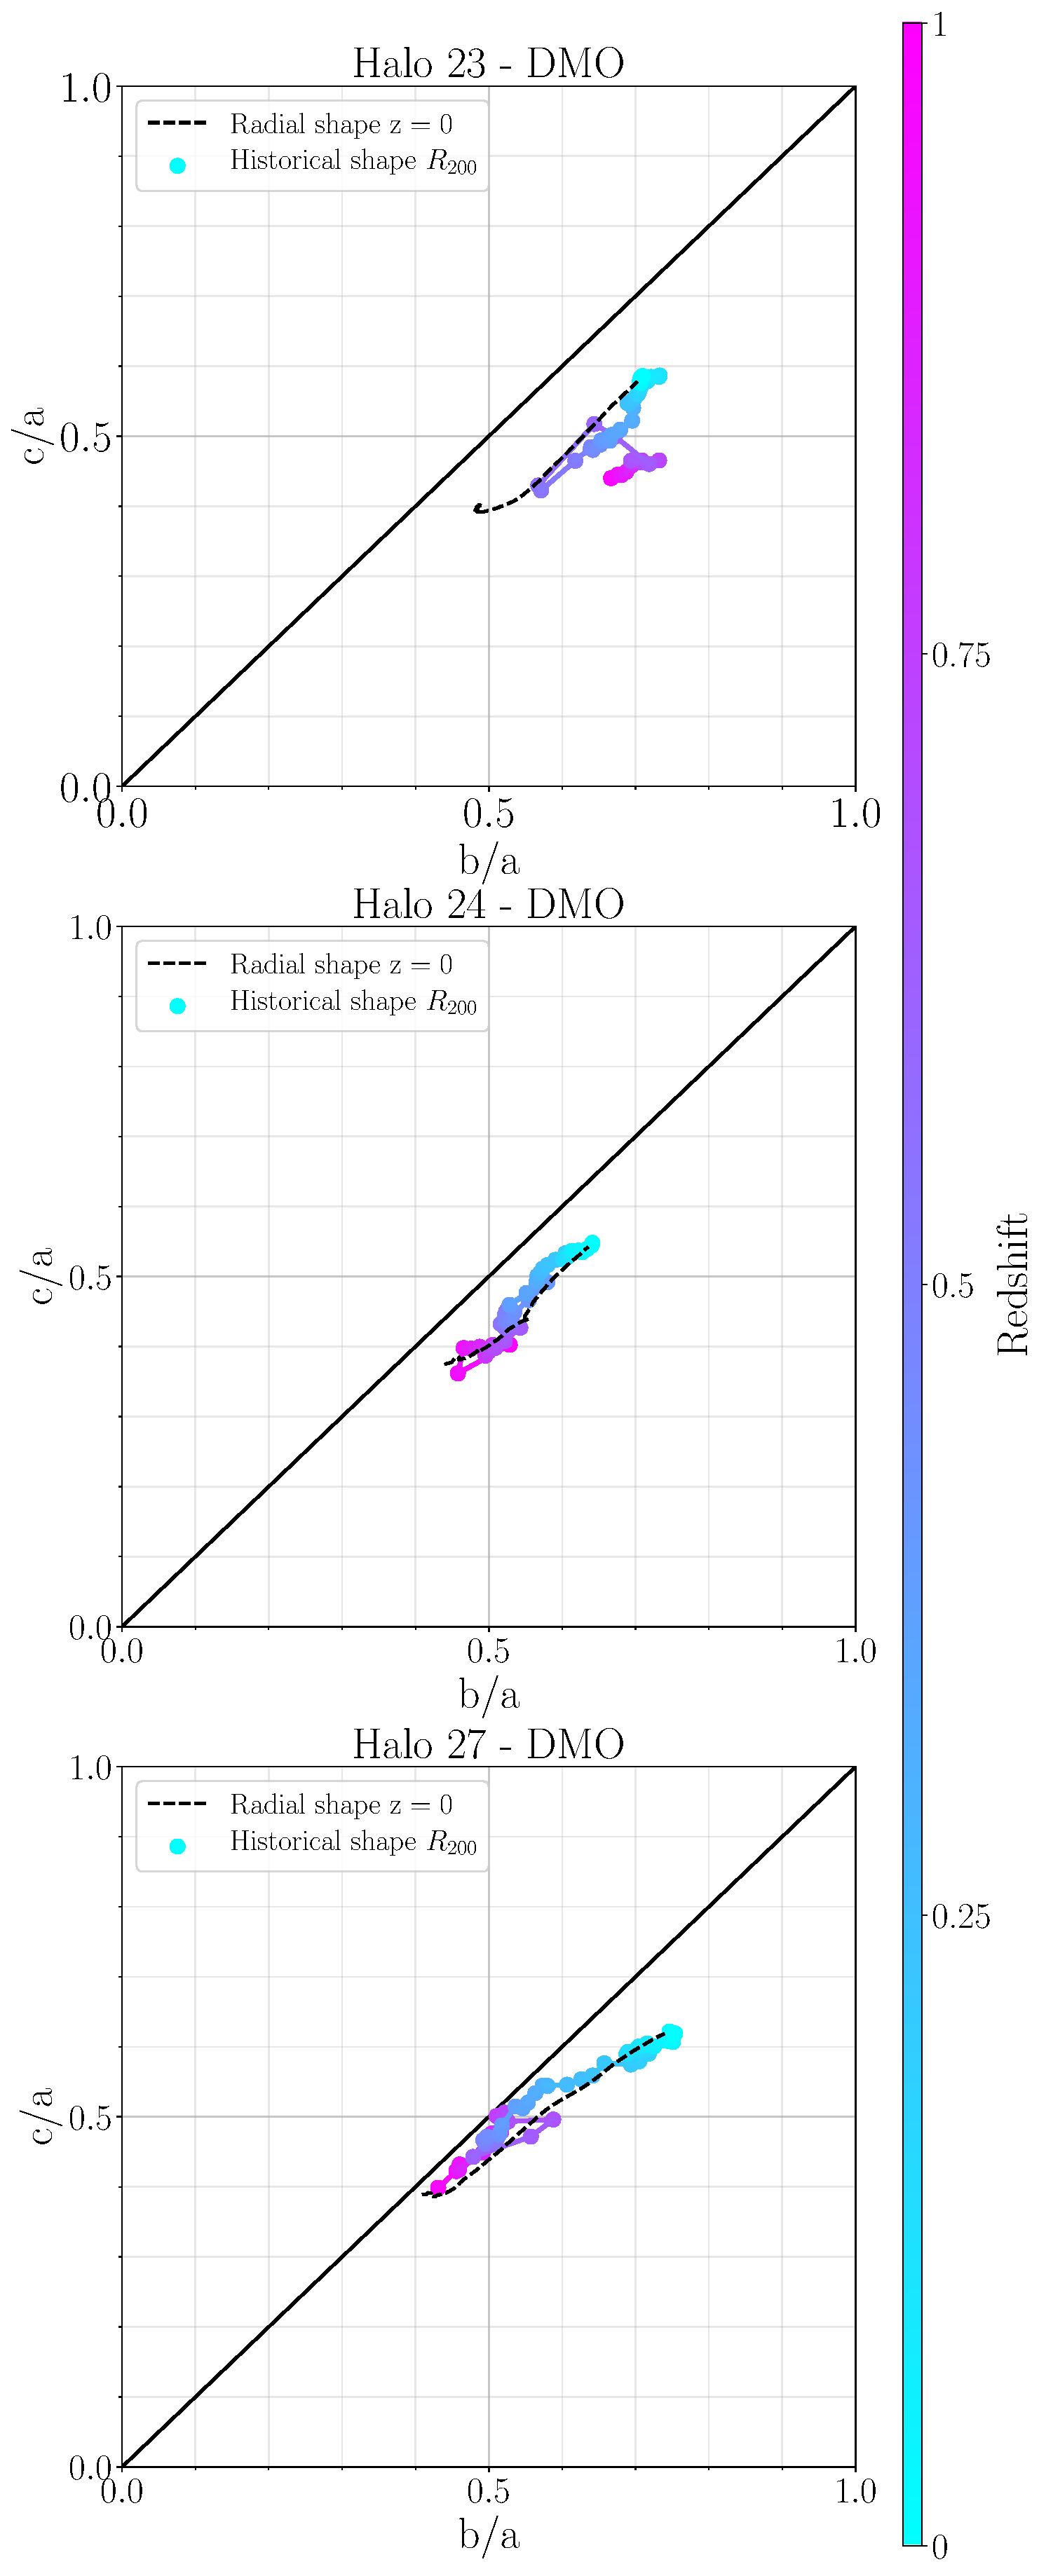
\includegraphics[width=0.35\textwidth]{Z_Triax_level3_set_B_DM.pdf}
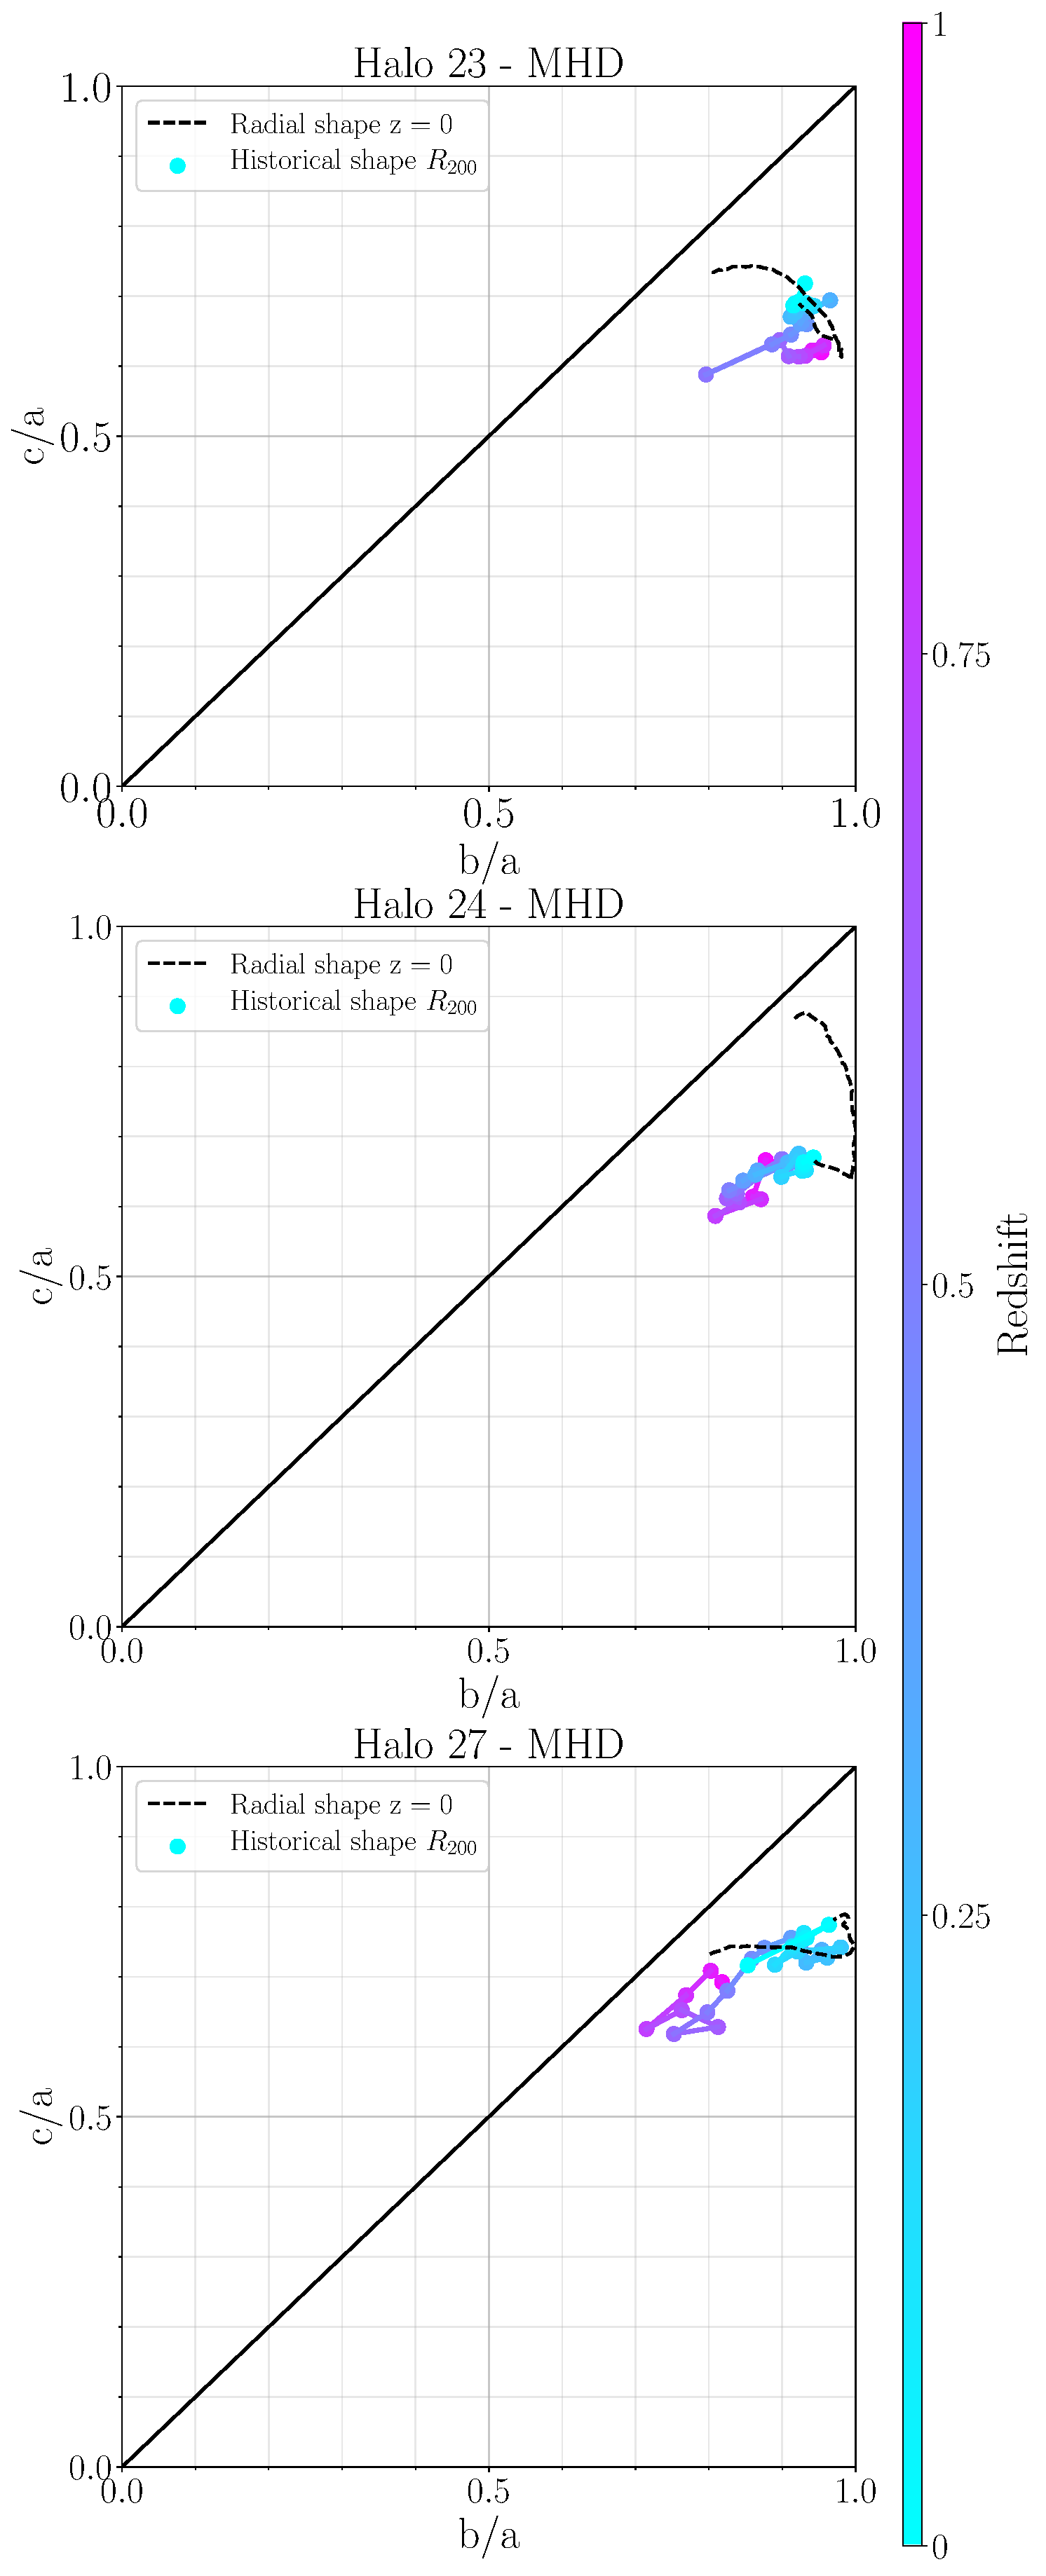
\includegraphics[width=0.35\textwidth]{Z_Triax_level3_set_B_MHD.pdf}
\end{center}
\caption{Same as Figure \ref{fig:triaxial_history_A}.
  These three halos correspond the second half of the sample for the
  \texttt{Level3} haloes. 
}
\label{fig:triaxial_history_B}
\end{figure*}

\begin{figure*}
\begin{center}
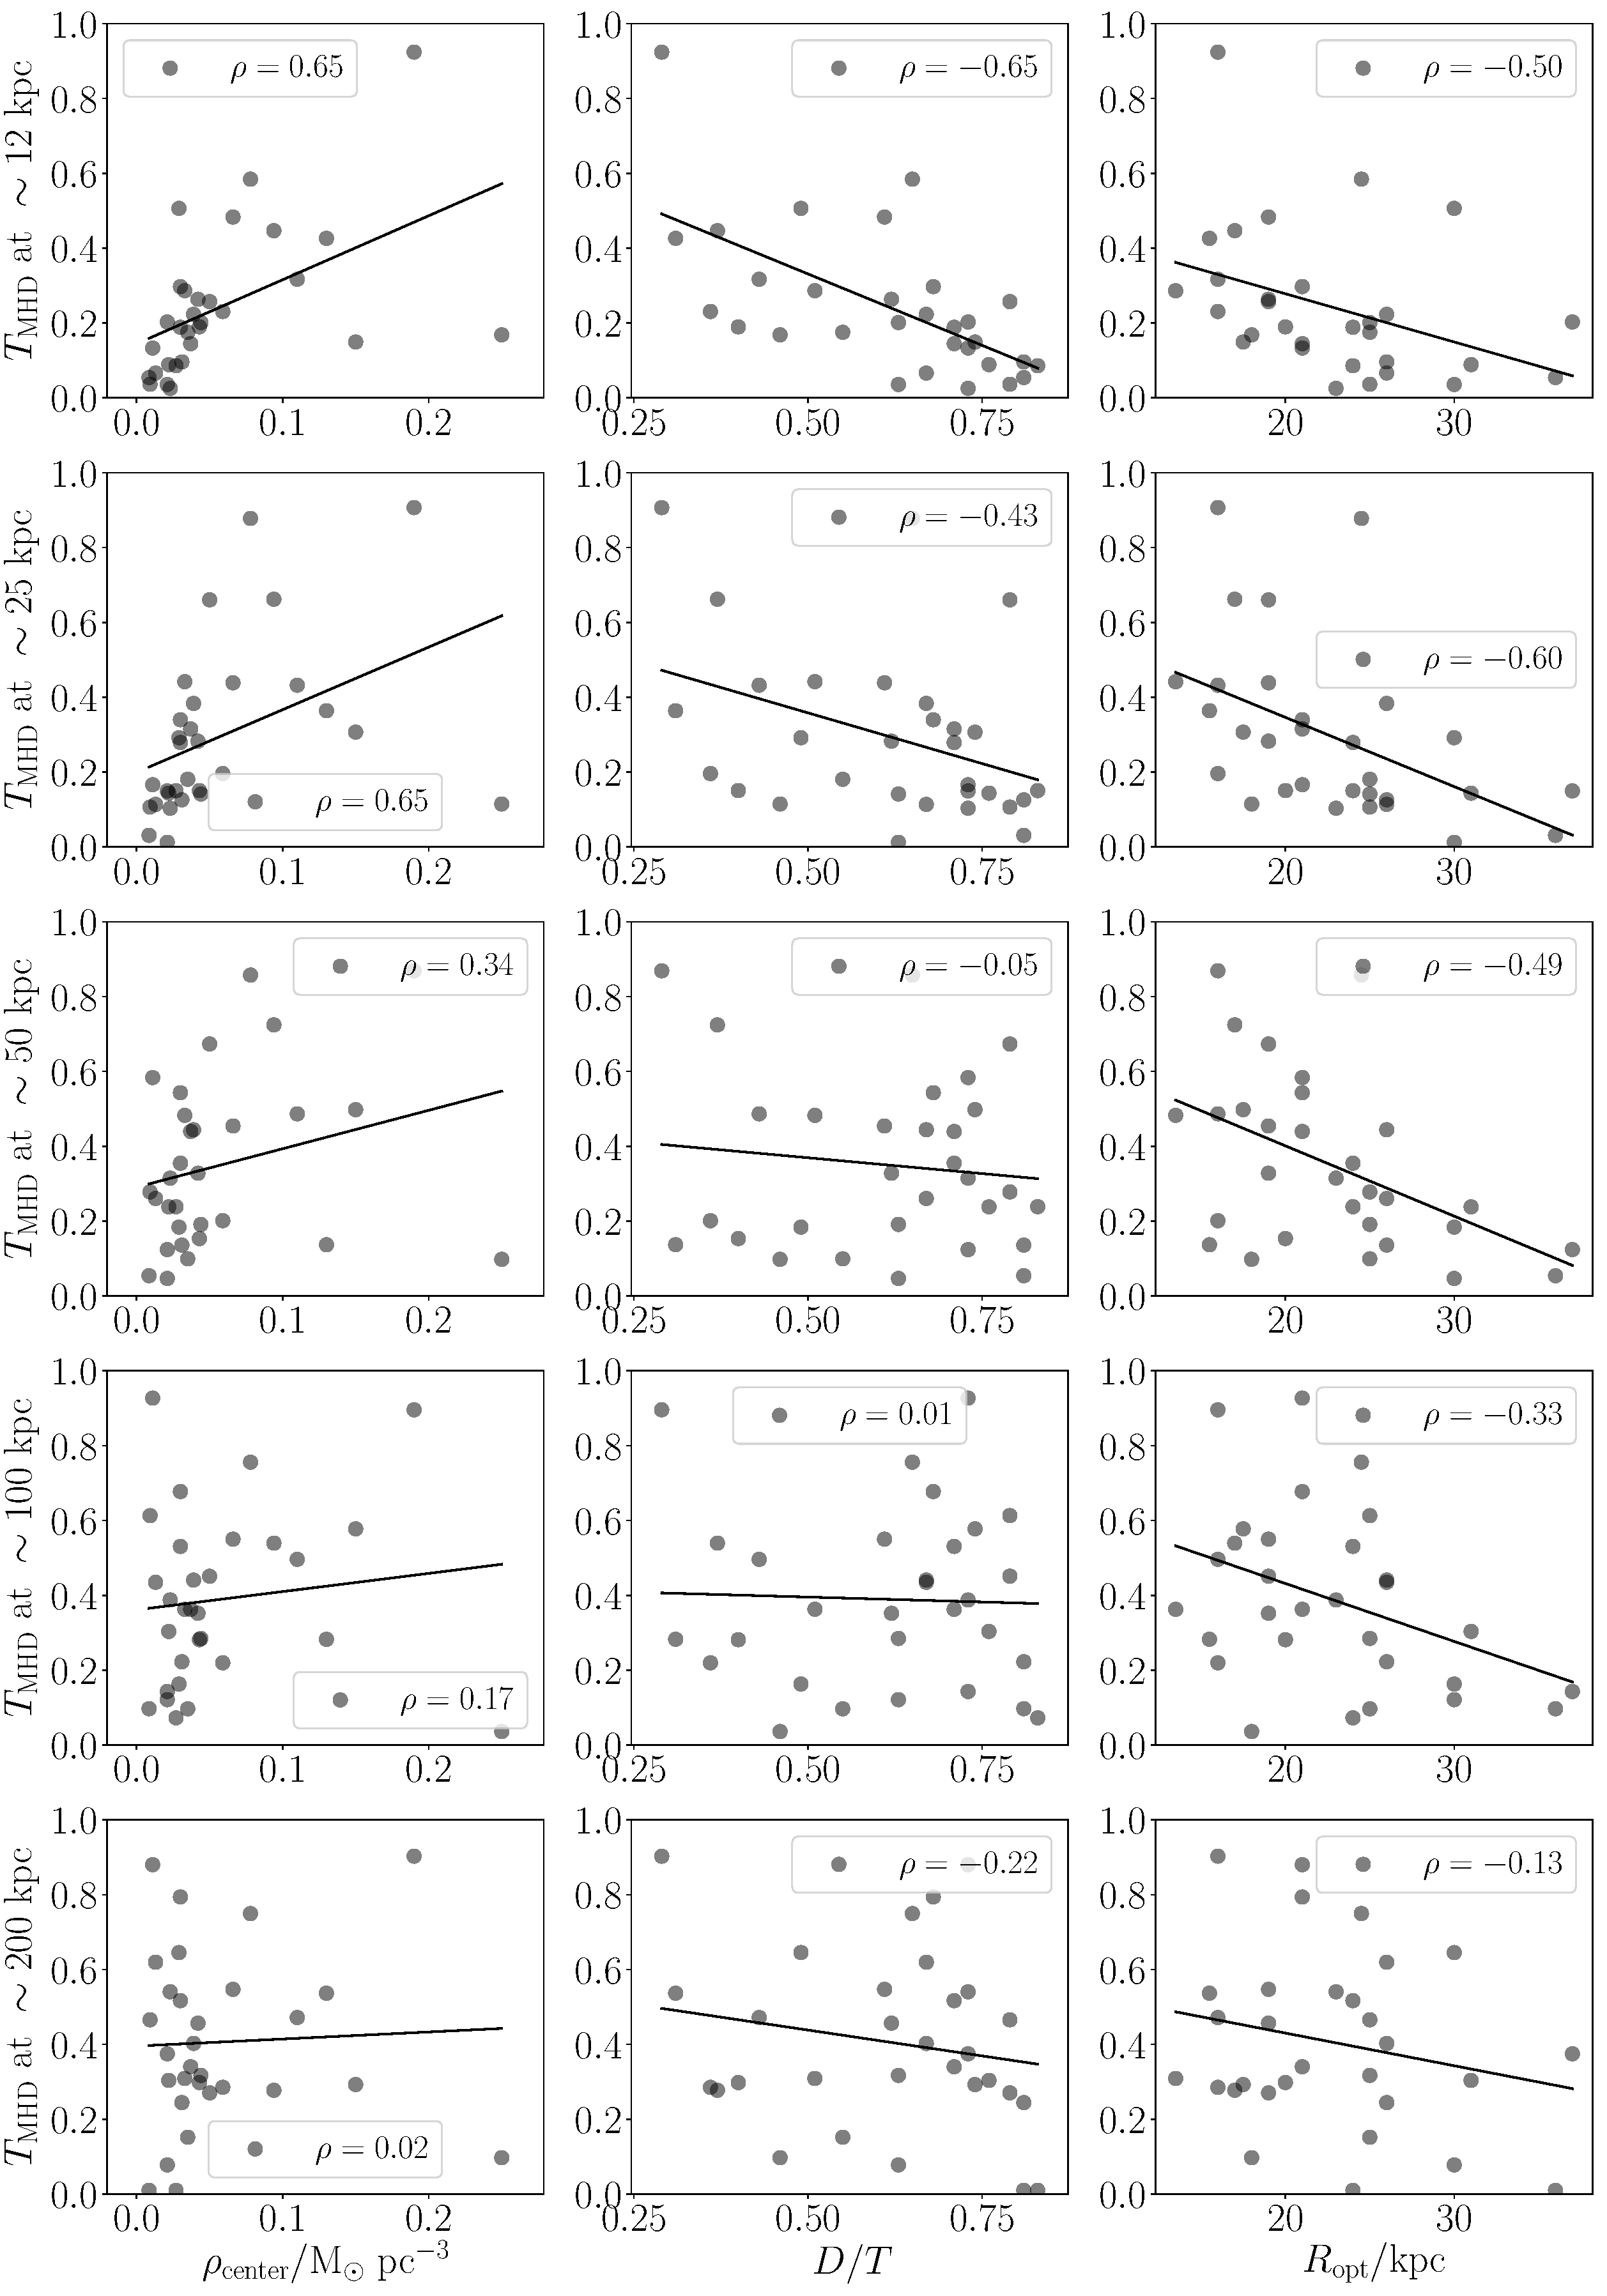
\includegraphics[width=0.8\textwidth]{correlation_T_MHD_disk.pdf}
\end{center}
\caption{Correlations between the halo triaxility at different radii
  and baryonic disk properties. 
  The label with the $\rho$ value corresponds to the Spearman's rank
  correlation coefficient.
  The line is the best linear minimum squares fit.
  The x-axis in the first column is the gas density at the center of
  the galaxy with in a sphere of radius  $1$ kpc \citep{Pakmor17};
  the second column shows the disk to total mass ratio and the last
  column includes the disk optical radius defined to be the radius at which the
  $B$-band surface brightness drops below 25 mag arcsec$^-2$ \citep{auriga}.
  The largest correlations are found for the two smaller radii and
  dilute as one approached $R_{200}$.
  Large and massive stellar disks with a low gas content are
  correlated with low dark matter triaxilities.}
\label{fig:disk_correlations}
\end{figure*}


\begin{figure}
\begin{center}
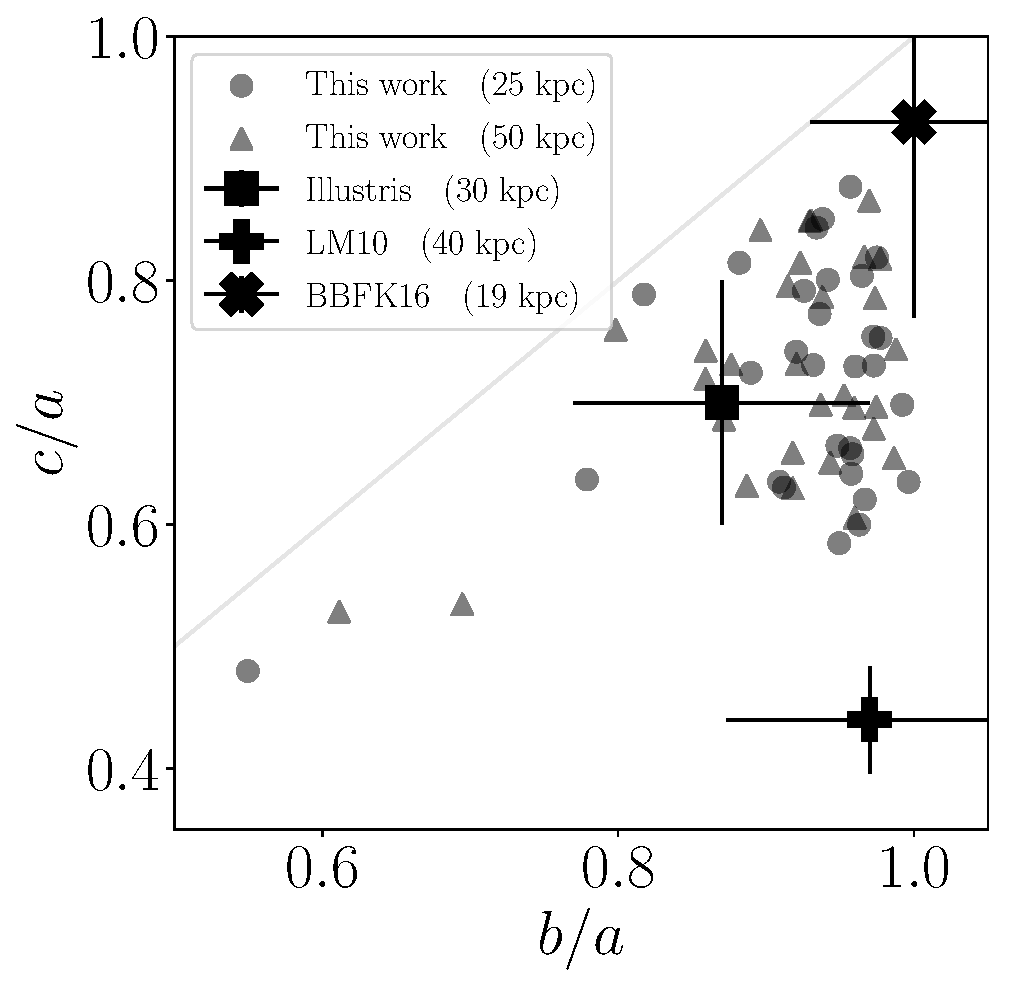
\includegraphics[width=0.45\textwidth]{triaxiality_observations.pdf}
\end{center}
\caption{Comparison of our results against other simulations
  by \citet{Chua19} (Illustris) and observational constraints for the 
dark matter halo shape in the Milky Way by \citet{LM10} (LM10) and
\citet{Bovy16} (BBFK16).   
We report our results in the MHD simulations in such a way as to
bracket the radii in the other estimates.
We find that our results are broadly consistent with the Illustris
simulations given the broad dispersion in both data sets.
The consistency with the constraints by \citet{Bovy16} is marginal,
only 1/5 of the halos in our sample seem to be consistent within the
observational reults.
The result by \citet{LM10} would place the Milky Way halo as an
atypical object in the $\Lambda$ CDM context.} 
\label{fig:observations}
\end{figure}


\section{Halo Shape Measurement}


The DM halo shape at a fixed radius is an estimate of either
the isopotential or isodensity surfaces.  
Observational inference models usually estimate the 
isopotential contours which are probed by tracers (gas, stars), while
simulations work with the isodensity contours which can be directly
calculated from particle positions.  
Furthermore, the density contours in thin shells are very sensitive to
the presence of small satelites.  
For this reason we measure the shape by taking
volume-enclosed particles, rather than shell-enclosed.  
This method yields results in good agreement to the isodensity
contours in the inner halo region, roughly for radii smaller than one
quarter the virial radius as explored by
\citep{Vera-Ciro_et_al._2011}. 

We measure the shape using the reduced inertia tensor \citep{Allgood_et_al._2006}, 


\begin{equation}
I_{ij} = \sum_k \frac{x_k^{(i)}x_k^{(j)}}{d^2_k},
\label{eq:inertia}
\end{equation}

where the particle positions are measured from the minimum of the
gravitational potential in each halo and each is weighted by the k-th
particle distance 
$d_k^2=x_k^2+y_k^2+z_k^2$.

The diagonalization of this tensor yields the eigenvectors and
eigenvalues that represent an ellipsoidal dark matter halo.
The axis lenghts of this ellipsoid $a\geq b \geq c$ are the square
root of the ${\bf I}$ eigenvalues and the direction of the principal
axis are the corresponding eigenvectors 

We start the calculations taking into account particles within a
sphere of radius $R$ and then recharacterize the triaxial parameters
by taking into account particles within an ellipsoid of semi-axes
$r,r/q,r/s$ and re-scaled distance $d^2=x^2+(y/q)^2+(z/s)^2$, where $q
= b/a$ and $s=c/a$ are the previously calculated axial ratios. 
We repeat this process until the average deviation of semi-axes is
less than $10^{-6}$.  
This is the same method used to estimate the halo shape in the DM-only
Aquarius simulations \citep{Vera-Ciro_et_al._2011}. 

Following the convergence critery by \cite{Vera-Crito_et_al.2011} we
restrict the sampling of the ellipsoidal parameters to radii  between
$\sim 2$kpc and $R_{200}$, where  $R_{200}$ correspond to the  radius
enclosing a sphere with 200 times the average dark matter density of
the Universe.  
On average, over the 30 halos in the \texttt{Level4} sample
$R_{200}=200\pm 10$kpc. 
For \texttt{Level3} halos we go down to distances $\sim 0.2$ kpc.  


\section{Results}

\subsection{The effect of baryons at $z=0$}

In the DMO sample we find that halos are rounder with increasing
radius.
The upper panels in Figure \ref{fig:slices} illustrates this effect.
The contours show a projected DM slice while the ellipsoid corresponds
to the full 3D shape determination. 
There we see a highly ellipsoidal halo shape at radii $\sim 3$kpc
that becomes less triaxial at $\sim 50$ kpc.


We summarize this trend in Figure \ref{fig:triaxiality_plane} by
plotting the results of all the 30 halos in the DMO sample.
The left panel shows every halo in the $c/a$-$b/a$ plane at
two different radii $R_{200}/8 (\sim 20$kpc$)$ and $R_{200}$. 
The outer part of the halo is systematically rounder tha its inner
region. 
Nevertheless the halo shape can still be considerated to be prolate at
all radii. 
These plots confirm the results already reported in the
literature \citep{Vera-Ciro_et_al._2011}.

A different picture presents itself in the MHD sample.
There all halos become rounder at all radii than its DMO
counterpart.
The lower panel in Figure \ref{fig:slices} can be directly compared to
its MHD counterpart; there we observe how at large radii the halo
becomes almost spherical. 
The right panel in Figure \ref{fig:triaxiality_plane} shows the
results for the 30 halos in the MHD sample.
This time the bulk of the halos can be considered oblate and close to
spherical. 

In Figure \ref{fig:triaxial_cumulative} we summarize the results at
different radii using the cumulative distributions for the 
triaxility parameter $T$ defined as 
\begin{equation}
T=\frac{a^2-b^2}{a^2-c^2}.
\label{eq:triaxiality}
\end{equation}
The left panel of this Figure shows that in the DMO sample the
triaxility has a median larger than $0.5$ at all radii, furthermore
this median value increases as we move towards the inner part of the
halo.
The right panel shows the exact complementary picture in the MHD
sampe.
There the median triaxility is alwas smaller than $0.5$ and this
triaxility is smaller as we move closer to the galactic disk.


Next we want to test to what extend the global effect of decreasing
triaxility in MHD simulations compared to the DMO sample 
holds for individual halos. 
We compute $\Delta T\equiv T_{\rm MHD}-T_{\rm DMO}$ the difference between the
triaxility in the MHD and the DMO simulation for each individual halo. 
Figure \label{fig:delta_triaxial_cumulative} shows the cumulative
distribution at the same radii as in
Figure \label{fig:delta_triaxial_cumulative}. 
    





\subsection{Shape evolution with cosmic time}

In the previous section we stablished that DMO halos at $z=0$ have
a steady and monotenouse trend towards decreasing triaxility with
increasing radius.
\cite{Vera-Ciro_et_al._2011} found that this  radial trend at $z=0$ 
correlates with the halo shape as a function of cosmic time, i.e.
the halo becomes less triaxial as cosmic time progresses. 
This correlation was interpreted as each radial shell retaining memory
of the accreting conditions at the virial radius at the time of
collapse.

Here we use the six \texttt{level3} halos to measure to what extent
the presence of baryons affect this memory effect.
The left column of Figure \ref{fig:redshift_triaxial} shows the six
halos in the triaxility plane. 
The colour dots show the time evolution while the black line
corresponds to the radial trend at $z=0$.
The close overlap of the spatial and temporal trends confirms the
memory effect found by \cite{Vera-Ciro_et_al.2011}.


In the MHD sample the memory effect is less evident. 
The right column of Figure \ref{fig:redshif_triaxial} shows the
corresponding results for the six halos in the MHD sample.

%Discuss if this correlation may be recovered if compared for example
%at Disk radius in stead of virial radius.\\ 


\subsection{DM halo - Stellar Disk Alignment}


A common assumption in observational models of the MW DM halo is that
its minor axis is perfectly aligned with the disk axis.
Although it is a reasonable assumption to guarantee the
stability of the galactic disk in simplified models of isolated
galaxies, this might not hold in an explicit cosmological context.

To examine the validity of this assumption  we sampled the shape at 5
different radii and plotted  directions in a cartesian coordinate
system where the $z$-axis always corresponds to the minor axis
measured at the virial radius.

{\bf En este caso hace falta la figura con la distribuci\'on integrada de cos theta}.
Figure \ref{fig:alignment} shows the cumulative distribution of
$\cos\theta$, where $\theta$ is the angle betwen the DM halo minor
axis and the stellar disk angular momentum.  
Each line shows the results at different radii.
We find that the majority of the disks are aligned with the minor axis
of their DM halo within $\approx 30^{\circ}$. 
Furthermore, if there is a good alignment measured at the virial
radius, this alignment is well conserved at smaller radii.

{\bf En este caso hace falta la figura de la evoluci\'on de cos theta
  como funci\'on del redshift}
However, there are some disks that show strong missalignments. 
To better understand the missalignments we plot the evolution of
$\cos\theta$ with time to find that the missalignment has been present
for the last XXX Gyr.
This trend is summarized in Figure \ref{fig:alignment_history}.


\section{Discussion}


\subsection{What drives the rounding effect?}

From our characterization of radial shapes it is clear that
MHD halos are rounder than DM halos every sampled radii. 
It is also noticeable that the rounding effect of baryons is stronger
at the disk regime, where the DM halo is almost perfectly oblate. 
Furthermore, MHD halos tend towards more oblate shapes (T < 0.5)
despite DM halos tendency towards more prolate shapes (T>0.5). 
This rounding effect can be explained by gravitational effect of the
flattened axisymmetric galactic disk. 
It also explanes the weakness of this affect around $\approx 100$kpc,
where the disk potential is weaker compared to the DM halo potential. 

Following that linea reasoning, one would also expect that the rounding
effect of baryons is related to some  galactic parameters such as its
component masses and radii. 
We look for these kind of correlations and to find that the strongest
can be found for the stellar density.
However, the correlation is relatively low ({\bf cuanto vale el
  coeficiente de correlation}) most likely due to the different
formation histories.
In other words, the effect of the baryonic disk on the shape of the DM halo
does not fully explain the deviation from oblateness of MHD halos at
$r<10$kpc. 

{\bf Finalmente cuales son las cantidades disponibles en el disco?
  cuales son las que muestran una mayor correlacion? Haria falta un
  plot con todas las correlaciones y la mencion de alguna prueba de
  machine learning del fit lineal para ver cuales son los parametros
  mas importantes.}
  
  We measured the sphericity of a halo shape defined as the distance 
  from the point that characterizes the shape in the triaxiality plane
  to the point $(q=1,s=1)$, which represents a perfect sphere. Taking this 
  as our metric of interest, the sphericity question becomes a search for
  important variables and tendencies that affect this quantity. For this case,
  given the small sample of 30 halos, we chose to study this problem with different 
  3 methods to account for the lacking statistical consistency. We analyzed the effect
  of the Star disk Radius, Baryonic fraction, Gas density, BH density, Gas Radius and
  Star density.\\
   
  We started with a simple linear Lasso regression to force a classification of 
  important variables. Then, we converted this problem in a binary classification problem
  by partitioning the samples in two balanced groups according to the studied metric which was then fitted using Random forest.
  Finally, we concluded this analysis with an MCMC sampling of the likelyhood of a linear model
  with varying slope and intercept parameters.\\
  
  The results of each method are presented below:


\textit{ Talk about source of triaxiality at the inner parts of the
  halos (bar?). This source of triaxiality at the inner parts explains
  why the axial ratios are $\approx 0.95$ and not exactly $1$. We
  should also discuss that the decrease in the axial ratios for bigger
  radii may actually be bigger/steeper but it is dimmed by the
  contribution of inner parts.} 


%\begin{figure}
%  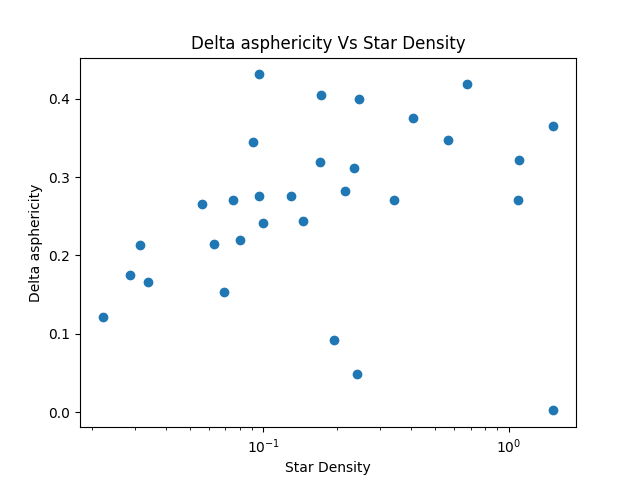
\includegraphics[width=\columnwidth]{./pics/Delta asphericity Vs Star Density.png}
%  \caption{Difference in asphericities between MHD and DM shapes Vs
%    Star Density of the simulation. Unsure about this graphic. Take
%    delta asphericity as the strength of the rounding effect of
%    baryons.}  
%  \label{fig:Star_Density_effect}
%\end{figure}




Half of the observational constraints are computed in terms of
isodensity contours, the other half in terms of isopotential contours.
To compare our results against the second kind we must either
translate the isodensity results or recompute in terms of isopotential
regions.
For this purpose, we run a simple iterative algorithm to find an
approximation of the shape of the isopotential contour. 

First, we calculate the mean and standard deviation of the potential over a
spherical shell of width equals to $10\%$ of the radius at which it is
sampled. 
Then, we calculate the inertia tensor of particles with potential
within $1\sigma$ around the mean potential and calculate its triaxial
characterization with the reduced inertia tensor. 
We repeat the
process of calculating the potential mean and standard deviation until
convergence is achieved with tolerance of $10^{-4}$. 

In Figure \ref{fig:density_potential} we compare the two approaches to
measure the axial rations and plot the analytic expectation for $q$, 
$(1-q_{\phi})\approx \frac{1}{3}(1-q_{\rho})$
\citep{Binney_and_Tremaine_2008}, taking the volume-enclosed axial
ratios  as an approximation for the isodensity contour ratios
$q_{\rho}$. 
This plot is computed at four different radii.

Although the analytic expression is meant to be used on the outer
regions of logarithmic axisymmetric halos, it works well as a first
approximation for nearly axisymmetric halos as those produced by our
simulations 
We find that the difference between the measured and the
approximated isopotential axial ratios is not bigger than $quantity
percent$.


\section{Conclusions}


\section*{Acknowledgements}
This project has received funding from the European Union's Horizon
2020 Research and Innovation Programme under the Marie
Sk\l{}odowska-Curie grant agreement No 734374. 

 \bibliographystyle{mnras}
 \bibliography{references}
\end{document}
